\begin{frame}
	\frametitle{Algoritmos baseados em grafos}
	\par Essa estrutura pode ajudar na resolução e modelagem de vários problemas como o de ordenação como já foi vista com o \textit{heap-sort}, de busca como na \textit{árvore binária}, modelagem de mapas, relacionamentos em redes de pessoas ou computadores, etc.
	\par Os relacionamentos podem ser de:
	\begin{itemize}
		\item conexão ( o que se conecta com o que )
		\item precedência ( o que vem antes do que )
		\item exclusão mutua ( como as coisas se agrupam? elas tem ligação? )
		\item prefêrência ( o que se encaixa melhor e onde )
	\end{itemize}
\end{frame}

\begin{frame}
	\frametitle{Algoritmos baseados em grafos}
	\par Grafos $G$ são estruturas que representam relacionamentos par-a-par entre pontos ou objetos. Os pontos são os \textbf{vértices ou nós} e as \textbf{arestas} (ou arcos quando são direcionais) são os relacionamentos. \textbf{Neste material}, ao conjunto dos vértices daremos o nome de $V(G)$ e ao conjunto das arestas nomearemos como $A(G)$.
	\begin{columns}
		\begin{column}{0.3\textwidth}
			\begin{figure}
				\centering
				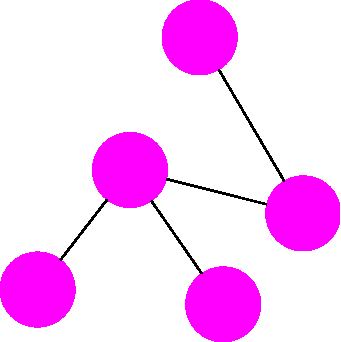
\includegraphics[width=0.9\linewidth]{images/grafoGenerico}
				\caption{Um grafo}
				\label{fig:grafogenerico}
			\end{figure}
		\end{column}
		\begin{column}{0.7\textwidth}
			\begin{itemize}
				\item se $\{a,b,c,d,e,f,g,h,i\}$ são vértices de um grafo então $G = \{a,b,c,d,e,f,g,h,i\}$
				\item se $a = uv / u \in G, v \in G \therefore  a = aresta \in A(G)$ então:
				\begin{itemize}
					\item $u, v$ são adjacentes
					\item $u, v$ são extremos de $a$
					\item $a$ passa por $uv$ e $a$ é delimitada por $u, v$
				\end{itemize}
				\item Se $u \in V(G)$ o grau de $u$ é a quantidade de vizinhos $d_G(u)$
				\item o grau mínimo é $\delta(G)$ e o máximo é $\Delta(G)$
				 \item $\sum_{v \in V(G)} d_G(v) = 2.|A(G)|$, ou seja, a soma dos graus é igual a duas vezes o total de arestas 
			\end{itemize}
		\end{column}
	\end{columns}
\end{frame}

\begin{frame}
	\frametitle{Algoritmos baseados em grafos}
	\framesubtitle{Grafos simples}
	\begin{itemize}
		\item não tem arestas paralelas (duas arestas ligando o mesmo par de vértices)
		\item laços (um vértice ligado a ele mesmo)
	\end{itemize}
\end{frame}

\begin{frame}
	\frametitle{Algoritmos baseados em grafos}
	\framesubtitle{Digrafos}
	\begin{columns}
	\begin{column}{0.5\textwidth}
		\par Quando a lista dos vértices não é suficiente para representar  as relações entre os mesmos e essas dependem de uma \textbf{procedência} se pode usar os digrafos como representação de tal situação. Um digrafo é um conjunto de dois outros conjuntos onde o primeiro representa os vértices e o segundo contém \textbf{pares ordenados} indicando as relações de precedência.
		
		\begin{equation}
			\begin{aligned}	
				D=	
				\begin{cases}
					V(G) = \{a,b,c,d,e,f,g\} \\
					A(G) = \{ab,bg,ce,de,fg\}
				\end{cases}
			\end{aligned}
		\end{equation}

	\end{column}
	\begin{column}{0.5\textwidth}
			\par Se $ a = uv $ é um \textbf{arco} de $D$ então:
			\begin{itemize}
				\item $u$ é cabeça e $v$ é a cauda
				\item $a$ sai de $u$ e vai para $v$
				\item o grau de entrada $d^-_D(u)$ de $u$ é a qtde de arcos que entram em $u$
				\item o grau de saída $d^+_D(u)$ de $u$ é a qtde de arcos que saem de $u$
				\item a vizinhança de entrada de $u$ é o conjunto de todos os vértices que entram em $u$, $N^-_D(u)$
				\item a vizinhança de saída de $u$ é o conjunto de todos os vértices que saem de $u$, $N^+_D(u)$
			\end{itemize}
		\end{column}
	\end{columns}
\end{frame}

\begin{frame}
	\frametitle{Algoritmos baseados em grafos}
	\framesubtitle{Digrafos}
	\par Para qualquer digrafo $D$ vale:
	\begin{itemize}
		\item $ \sum_{v \in V(D)} d_D^+(v) = \sum_{v \in V(D)} d_D^-(v) = |A(D)| $, ou seja, a soma total de todos os graus de saída é igual a soma de todos os graus de entrada que é igual ao número total de arcos.
		\item Todo digrafo pode gerar um grafo subjacente que nada mais é do que um grafo sem suas direções.
		\item Todo grafo pode ser a base de construção de um \textbf{digrafo associado} $D(G)$ adicionando-se \textbf{arcos paralelos} a cada par de vértices. Ao digrafo que não usa arcos paralelos chamaremos de \textbf{digrafo orientado} $\overrightarrow{G}$.
		\item Os arcos podem ter associados a eles valores $w(uv)$ que serão chamados de \textbf{pesos}.
	\end{itemize}
\end{frame}

\begin{frame}
	\frametitle{Algoritmos baseados em grafos}
	\framesubtitle{Digrafos}
	\par No entanto, na maioria das vezes, representaremos grafos e digrafos da mesma forma pois, mesmo que não haja relações de precedência entre os nós, é preciso indicar as arestas de tal grafo. 
\end{frame}

\begin{frame}
	\frametitle{Algoritmos baseados em grafos}
	\framesubtitle{Representações}
	\par Como já foi visto um grafo pode ser representado por um vetor simples desde que o algoritmo que o trata seja projetado devidamente para usar esta estrutura. No entanto, nem sempre é prático, possível ou eficiente usar uma estrutura tão simples, portanto temos que usar outros tipos:
	\begin{itemize}
		\item lista de adjacências: São listas que, dado um vértice, contém uma \textbf{lista ligada} que contêm todos os vizinhos daquele nó ou, no caso dos digrafos todos os nós de saída daquele vértice.
		\item matrizes de adjacências: É uma \textbf{matriz quadrada} de dimensão igual a quantidade de vértices do grafo na qual a linha $u$ que se cruza com a coluna $v$ indicam se tais vértices são adjacentes.
	\end{itemize}
\end{frame}

\begin{frame}
	\frametitle{Algoritmos baseados em grafos}
	\framesubtitle{Representações: Lista de adjacências}
	\begin{columns}
	\begin{column}{0.6\textwidth}
		\begin{figure}
			\centering
			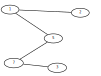
\includegraphics[width=0.4\linewidth]{images/listasDeAdjacencias}
			\caption{Ponteiros em rosa, lista ligada em verde}
			\label{fig:listasdeadjacencias}
		\end{figure}
		\par Memória ocupada: $V(G)$ ponteiros + $2.A(G)$ itens de lista ligada =  $\Theta(V(G) + A(G))$
		\par Tempo de busca por adjacências: $\Omega(1), O(n)$
		\par Bom para grafos esparsos com poucas arestas pois, se $V(G) = n \implies A(G) = \dfrac{n.(n+1)}{2} \implies O(n^2)$ de memória.
	\end{column}
	\begin{column}{0.4\textwidth}
		\begin{figure}
			\centering
			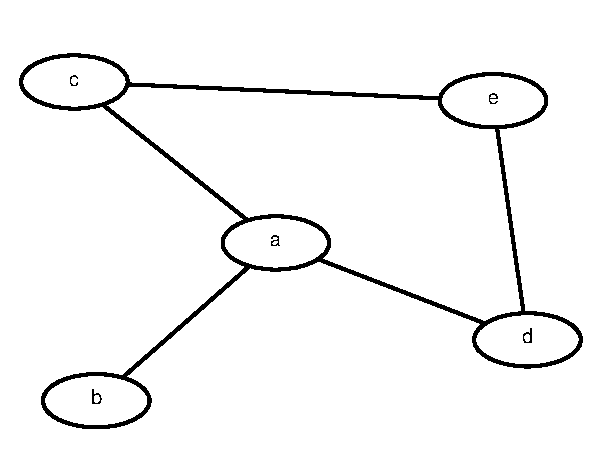
\includegraphics[width=\linewidth]{images/listasDeAdjacenciasGrafo}
			\caption{Exemplo de grafo}
			\label{fig:listasdeadjacenciasgrafo}
		\end{figure}
	\end{column}
\end{columns}
\end{frame}

\begin{frame}
	\frametitle{Algoritmos baseados em grafos}
	\framesubtitle{Representações: Matriz de adjacências}
	\begin{columns}
		\begin{column}{0.4\textwidth}
		\begin{figure}
			\centering
			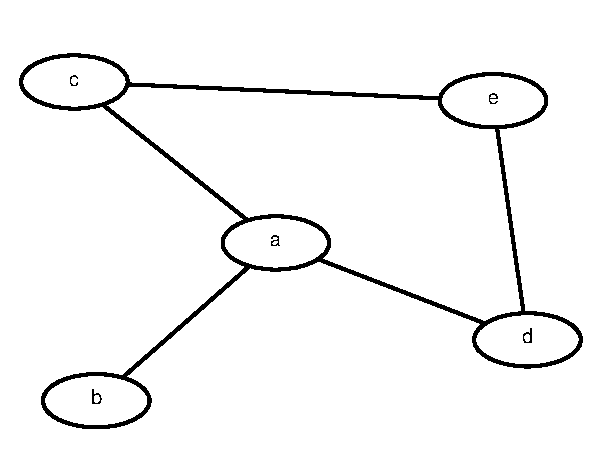
\includegraphics[width=\linewidth]{images/listasDeAdjacenciasGrafo}
			\caption{Exemplo de grafo}
			\label{fig:listasdeadjacenciasgrafo2}
		\end{figure}
		\end{column}
		\begin{column}{0.6\textwidth}
			\begin{equation}
				\left[
				\begin{matrix}
					& \mathbf{a}&\mathbf{b}&\mathbf{c}&\mathbf{d}&\mathbf{e} \\
					\mathbf{a}& 0&1&1&1&0 \\
					\mathbf{b}& 1&0&0&0&0 \\
					\mathbf{c}& 1&0&0&0&1 \\
					\mathbf{d}& 1&0&0&0&1 \\
					\mathbf{e}& 0&0&1&1&0 \\
				\end{matrix}
				\right]
			\end{equation}
			
			\par Na matriz as arestas $ab$, $bc$ e $dc$ são representadas.\newline
			\par Memória ocupada: $\Theta(n^2)$ para todos os casos.
			\par Tempo de busca por adjacências: $\Theta(1)$
			\par Melhor para grafos muito densos.
		\end{column}
	\end{columns}
\end{frame}

\begin{frame}
	\frametitle{Algoritmos baseados em grafos}
	\framesubtitle{Exercício 0}
	\par Represente os conjuntos do grafo abaixo, informe o grau de cada nó, represente a matriz de adjacências e a lista de adjacências.
		\begin{columns}
		\begin{column}{0.6\textwidth}
			\begin{figure}
				\centering
				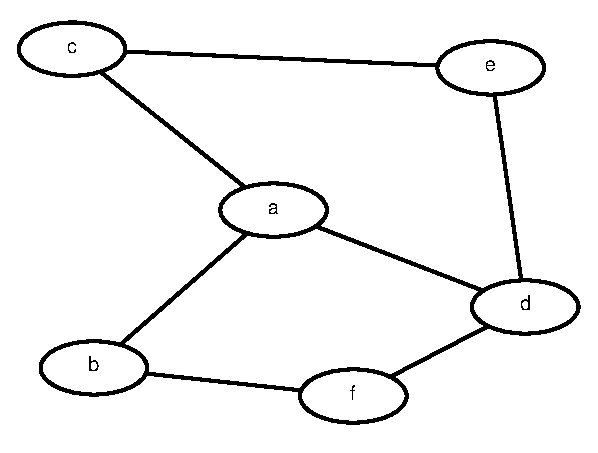
\includegraphics[width=.8\linewidth]{images/listasDeAdjacenciasGrafo2}
				\caption{Outro exemplo de grafo}
				\label{fig:listasdeadjacenciasgrafo3}
			\end{figure}
		\end{column}
		\pause
		\begin{column}{0.4\textwidth}
			\par \textbf{Resposta}:
			\only<2>{
				\par $ V(G)  = \{a,b,c,d,e,f\} $
				\par $ A(G)  = \{ab,ac,ad,de,df,ce,fd,fb\} $
				\par $ d_G(a) = 3 $
				\par $ d_G(b) = 2 $
				\par $ d_G(d) = 3 $
				\par $ d_G(c) = 2 $
				\par $ d_G(e) = 2 $
				\par $ d_G(f) = 2 $
			}
			\only<3>{
			\begin{equation}
				\left[
				\begin{matrix}
					& \mathbf{a}&\mathbf{b}&\mathbf{c}&\mathbf{d}&\mathbf{e}&\mathbf{f} \\
					\mathbf{a}& 0&1&1&1&0&0 \\
					\mathbf{b}& 1&0&0&0&0&1 \\
					\mathbf{c}& 1&0&0&0&1&0 \\
					\mathbf{d}& 1&0&0&0&1&1 \\
					\mathbf{e}& 0&0&1&1&0&0 \\
					\mathbf{f}& 0&1&0&1&0&0
				\end{matrix}
				\right]
			\end{equation}
			}
			\only<4>{
				\par $ a \rightarrow b \rightarrow c \rightarrow d $
				\par $ b \rightarrow a \rightarrow f $
				\par $ c \rightarrow a  \rightarrow e $
				\par $ d \rightarrow e  \rightarrow f $
				\par $ e \rightarrow d \rightarrow c $
				\par $ f \rightarrow d  \rightarrow b $
			}
		\end{column}
	\end{columns} 
\end{frame}

\begin{frame}[allowframebreaks]
	\frametitle{Algoritmos baseados em grafos}
	\framesubtitle{Exemplo de lista de adjacências}
	\lstinputlisting[language=C++]{../codigo/listaDeAdjacencia.cpp}
\end{frame}


\begin{frame}
	\frametitle{Algoritmos baseados em grafos}
	\framesubtitle{Exercício 1}
	\par \textbf{Programe} em c ou c++ a \textbf{matriz de adjacências} e adicione os nós como representado abaixo:
	\begin{figure}
		\centering
		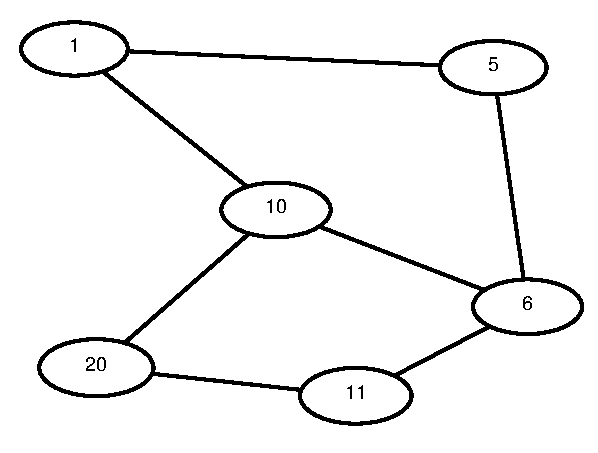
\includegraphics[width=.5\linewidth]{images/listasDeAdjacenciasGrafoExercicio}
		\caption{Outro exemplo de grafo}
		\label{fig:listasdeadjacenciasgrafo4}
	\end{figure}
\end{frame}

\begin{frame}
	\frametitle{Algoritmos baseados em grafos}
	\framesubtitle{Removendo vértices}
	\begin{columns}
		\begin{column}{0.4\textwidth}
			\par Até agora vimos como construir e como consultar algumas informações de um grafo mas e se precisarmos \textbf{remover} algum nó?
		\end{column}
		\begin{column}{0.6\textwidth}
			\begin{figure}
				\centering
				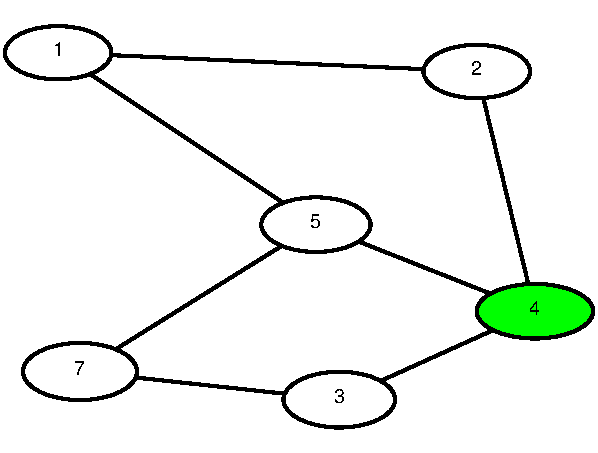
\includegraphics[width=0.8\linewidth]{images/remocaoDeVertice00}
				\caption{Remoção de vértice}
				\label{fig:remocaodevertice00}
			\end{figure}
		\end{column}
	\end{columns}
\end{frame}

\begin{frame}
	\frametitle{Algoritmos baseados em grafos}
	\framesubtitle{Removendo vértices - Matriz de adjacências}
	\begin{columns}
		\begin{column}{0.4\textwidth}
			\only<1>{
				\begin{equation}
					\left[
					\begin{matrix}
						 & \mathbf{1}&\mathbf{2}&\mathbf{3}&\mathbf{4}&\mathbf{5}&\mathbf{6}&\mathbf{7} \\
						\mathbf{1}& 0&1&0&0&1&0&0 \\
						\mathbf{2}& 1&0&0&1&0&0&0 \\
						\mathbf{3}& 0&0&0&1&0&0&1 \\
						\mathbf{4}& 0&1&1&0&1&0&0 \\
						\mathbf{5}& 1&0&0&1&0&0&1 \\
						\mathbf{6}& 0&0&0&0&0&0&0 \\
						\mathbf{7}& 0&0&1&0&1&0&0
					\end{matrix}
					\right]
				\end{equation}
				\par Basta essa representação para excluir um nó???
			}
			\only<2>{
				\begin{equation}
					\left[
					\begin{matrix}
						 & \mathbf{1}&\mathbf{2}&\mathbf{3}&\mathbf{\textcolor{green}{4}}&\mathbf{5}&\mathbf{6}&\mathbf{7} \\
						\mathbf{1}& 0&1&0&\textcolor{green}{0}&1&0&0 \\
						\mathbf{2}& 1&0&0&\textcolor{green}{0}&0&0&0 \\
						\mathbf{3}& 0&0&0&\textcolor{green}{0}&0&0&1 \\
						\mathbf{\textcolor{green}{4}}& \textcolor{green}{0}&\textcolor{green}{0}&\textcolor{green}{0}&\textcolor{green}{0}&\textcolor{green}{0}&\textcolor{green}{0}&\textcolor{green}{0} \\
						\mathbf{5}& 1&0&0&\textcolor{green}{0}&0&0&1 \\
						\mathbf{6}& 0&0&0&\textcolor{green}{0}&0&0&0 \\
						\mathbf{7}& 0&0&1&\textcolor{green}{0}&1&0&0
					\end{matrix}
					\right]
				\end{equation}
				\par Não! O nó continua existindo mas, sem ligação alguma.
			}
			\only<3>{
				\begin{equation}
					\left[
					\begin{matrix}
						 & \mathbf{1}&\mathbf{2}&\mathbf{3}&\mathbf{\textcolor{green}{4}}&\mathbf{5}&\mathbf{6}&\mathbf{7} \\
						\mathbf{1}& 0&1&0&\textcolor{green}{-1}&1&0&0 \\
						\mathbf{2}& 1&0&0&\textcolor{green}{-1}&0&0&0 \\
						\mathbf{3}& 0&0&0&\textcolor{green}{-1}&0&0&1 \\
						\mathbf{\textcolor{green}{4}}& \textcolor{green}{-1}&\textcolor{green}{-1}&\textcolor{green}{-1}&\textcolor{green}{-1}&\textcolor{green}{-1}&\textcolor{green}{-1}&\textcolor{green}{-1} \\
						\mathbf{5}& 1&0&0&\textcolor{green}{-1}&0&0&1 \\
						\mathbf{6}& 0&0&0&\textcolor{green}{-1}&0&0&0 \\
						\mathbf{7}& 0&0&1&\textcolor{green}{-1}&1&0&0
					\end{matrix}
					\right]
				\end{equation}
				\par Porém podemos introduzir um terceiro símbolo que dá conta do recado!
			}
		\end{column}
		\begin{column}{0.6\textwidth}
			\only<1>{
				\begin{figure}
					\centering
					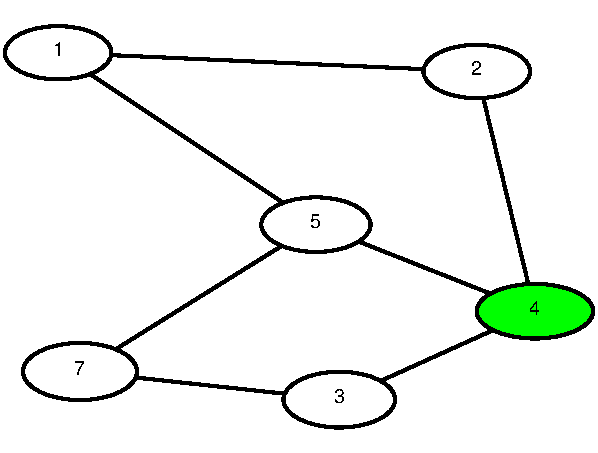
\includegraphics[width=0.8\linewidth]{images/remocaoDeVertice00}
					\caption{Remoção de vértice}
					\label{fig:remocaodevertice01}
				\end{figure}
			}
			\only<2>{
				\begin{figure}
					\centering
					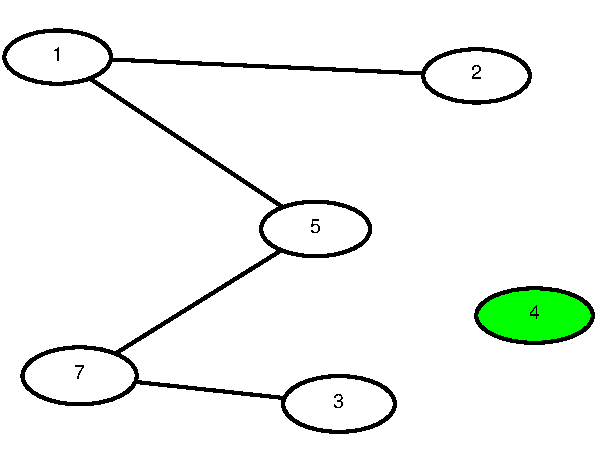
\includegraphics[width=0.8\linewidth]{images/remocaoDeVertice01}
					\caption{Remoção de vértice}
					\label{fig:remocaodevertice02}
				\end{figure}
			}
			\only<3>{
				\begin{figure}
					\centering
					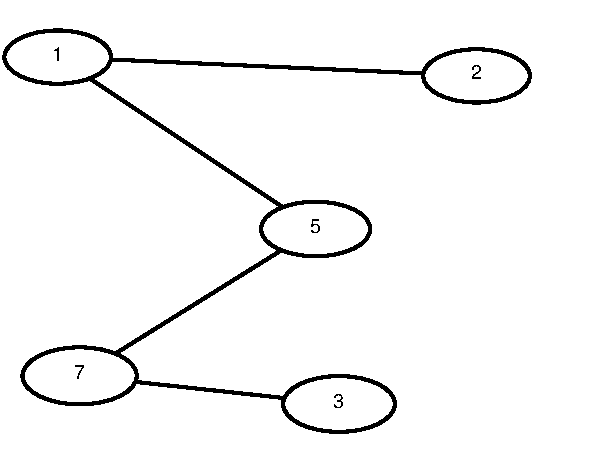
\includegraphics[width=0.8\linewidth]{images/remocaoDeVertice02}
					\caption{Remoção de vértice}
					\label{fig:remocaodevertice03}
				\end{figure}
			}
		\end{column}
	\end{columns}
\end{frame}

\begin{frame}
	\frametitle{Algoritmos baseados em grafos}
	\framesubtitle{Exercício 2}
	\par \textbf{Implemente} em c ou c++ a \textbf{remoção de nós} e a \textbf{remoção de arestas}
\end{frame}

\begin{frame}
	\frametitle{Algoritmos baseados em grafos}
	\framesubtitle{Subgrafos}
	\par Considere:
	\begin{equation}
		\begin{aligned}
			\begin{cases}
				&V(G) = \{a,b,c,d,e,f\} \\
				&A(G) = \{ab,ac,ad,dc,ef,fa,be\}
			\end{cases}
		\end{aligned}
	\end{equation}
	\par Então:
	\par Seja $u$ e $v$ dois vértices, um conjunto $H$ é subgrafo de $G$ se $V(H) \subseteq V(G), A(H) \subseteq A(G) / (u,v) \in V(H)$
	\par Um subgrafo $H$ é \textbf{gerador} se $H \subseteq G, V(H) = V(G)$
	\par Se $S \subseteq V(G), G[S]$ é o grafo induzido por $S$
	\par Se $F \subseteq A(G), G[S]$ é o grafo induzido por $F$\newline
	\par É importante notar que os subgrafos mantém as relações definidas anteriormente entre seus vértices.
\end{frame}

\begin{frame}
	\frametitle{Algoritmos baseados em grafos}
	\framesubtitle{Passeios}
	\par Passeios são operações cuja finalidade é visitar os vértices de um grafo, tal procedimento só é possível se houverem arestas entre os vértices visitados.
		\begin{equation}
		\begin{aligned}
			\begin{cases}
				&V(G) = \{a,b,c,d,e,f\} \\
				&A(G) = \{ab,ac,ad,dc,ef,fa,be\}
			\end{cases}
		\end{aligned}
	\end{equation}
	\par considerando o grafo acima \textbf{um dos} passeios possíveis é: 
	\par $P_1=\{a,b,e,f,a,c\}$
	\par O comprimento do passeio é dado pela \textbf{quantidade de vértices do mesmo}.
	\par Passeios fechados começam e terminam no mesmo vértice.
	\par Passeios abertos começam e terminam em vértices distintos. 
\end{frame}

\begin{frame}
	\frametitle{Algoritmos baseados em grafos}
	\framesubtitle{Passeios}
	\par Passeios que \textbf{não repetem} vértices são chamados de \textbf{caminhos}. Caminhos com $n$ vértices são chamados de $P_n$: $P_1, P_5, etc.$
	\par Passeios que \textbf{não repetem} vértices \textbf{exceto os extremos} são chamados de \textbf{ciclo}. Ciclos com $n$ vértices são chamados de $C_n$
	\par Passeios geram subgrafos.
	\par Grafos completos são aqueles nos quais existem arestas entre todos os vértices. Grafos completos com $n$ vértices são chamados de $K_n$: $A(K_n) = \dfrac{n(n-1)}{2}$
	\par $G$ é conexo se \textbf{todos} os pares de vértices são conectados por arestas.
	\par Em \textbf{digrafos} pode \textbf{ou não} ser verdade que $C_n =\{a, b, c, d\} \implies C_n^{'} =\{d, c, b, a\}$
	\par Em um \textbf{digrafo} se houverem caminhos entre quaisquer vértices $a \rightarrow b$ e $b \rightarrow a$ então esse digrafo é \textbf{fortemente conexo}.
\end{frame}

\begin{frame}
	\frametitle{Algoritmos baseados em grafos}
	\framesubtitle{Exercício 03}
	\par Crie exemplos que mostrem \textbf{todas} as propriedades dos \textbf{digrafos, grafos e seus respectivos subgrafos e passeios}.
\end{frame}

\begin{frame}
	\frametitle{Algoritmos baseados em grafos}
	\framesubtitle{Distâncias entre digrafos}
	\par A distância ($dist_G(u,v)$) entre dois vértices em um digrafo é dada pela quantidade de arestas de um vértice até o outro, se estes vértices não estiverem conectados então se diz que a distância é infinita ($\infty$).
	\par Lembre-se que a distância em grafos e digrafos pode variar sensivelmente.
	\par Em grafos e digrafos cujas arestas tem \textbf{pesos} a distância ($dist^w_G(u,v)$) é dada pelo \textbf{menor} valor da soma das arestas (menor distância).
\end{frame}

\begin{frame}
	\frametitle{Algoritmos baseados em grafos}
	\framesubtitle{O problema do caminho mínimo}
	\par O caminho mínimo é aquele que tem o menor valor de soma das arestas, atualmente esse problema só é possivel de se resolver se:
	\begin{itemize}
		\item o grafo não tem aresta com peso negativo
		\item o digrafo não tem um ciclo com peso negativo
	\end{itemize}
\end{frame}

\begin{frame}
	\frametitle{Algoritmos baseados em grafos}
	\framesubtitle{Exercício 04}
	\par Crie um algoritmo que calcula a distância mínima entre dois vértices.
	\par Qual o tempo de execução assintótico?
	\par Esse tempo é bom? Justifique.
\end{frame}

\begin{frame}
	\frametitle{Algoritmos de busca em grafos}
	\framesubtitle{Árvores}
	\par 
	Como já vimos anteriormente no algoritmo \textit{heap-sort} as vezes é necessário a implementação (seja na lógica ou em uma estrutura) de uma árvore mas, o que é uma isso? Assim como na natureza a árvore representa uma estrutura hierárquica na qual algumas partes se ligam a \textbf{uma} outra parte de forma recursiva formando assim uma estrutura parecida com que se pode chamar de fractal de linhas e nós. No contexto dos algoritmos de busca árvores são extremamente úteis pois, geralmente, diminuem muito o tempo para localização de um valor.
	
	\tikzset{
		tree/.style={
			every node/.style={rectangle,draw},
			level 1/.style={sibling distance=40mm},
			level 2/.style={sibling distance=20mm},
			level 3/.style={sibling distance=10mm},
		},
		fontbf/.style={font=\bfseries}
	}
	\begin{figure}
		\begin{tikzpicture}[tree]
			\node {20}
			child{
				node{10}
				child{node{5}}
				child{node{7}}
			}
			child{
				node{11}
				child{node{1}}
				child{node{2}}
			};
		\end{tikzpicture}
	\end{figure}
\end{frame}

\begin{frame}
	\frametitle{Algoritmos de busca em grafos}
	\framesubtitle{Árvores}
	
	\tikzset{
		tree/.style={
			every node/.style={rectangle,draw},
			level 1/.style={sibling distance=40mm},
			level 2/.style={sibling distance=20mm},
			level 3/.style={sibling distance=10mm},
		},
		fontbf/.style={font=\bfseries}
	}
	\begin{figure}
		\begin{tikzpicture}[tree]
			\node {20}
			child{
				node{10}
				child{node{5}}
				child{node{7}}
			}
			child{
				node{11}
				child{node{1}}
				child{node{2}}
			};
		\end{tikzpicture}
	\end{figure}
	\par Considerando que um grafo é dito \textbf{conexo} se existir \textbf{pelo menos um caminho entre cada par de vértices} do grafo. Se pode dizer que uma árvore é um \textbf{grafo conexo} que \textbf{não contêm ciclos} e, por consequência, cujo o número de arestas é o número de vértices - 1.
\end{frame}

\begin{frame}
	\frametitle{Algoritmos de busca em grafos}
	\framesubtitle{Árvores - Exercício 05}
	\par Dê exemplos de grafos que não são árvores.
\end{frame}

\begin{frame}
	\frametitle{Algoritmos de busca em grafos}
	\framesubtitle{Árvores - Propriedades}
	\par Se o grafo $G$ representa uma árvore ($T$) então \textbf{é equivalente} dizer que:
	\begin{itemize}
		\item existe um único caminho entre os dois vértices de $G$
		\item $G$ é conexo para toda aresta pertencente a $G$ $(a \in A(G))$ e remover um aresta o torna desconexo.
		\item é um \textbf{grafo conexo} que \textbf{não contêm ciclos} e, por consequência, cujo o número de arestas é o número de vértices - 1
		\item se $G$ não tem ciclos então todo par de vértices \textbf{não adjacentes} formará um ciclo caso se trace um aresta entre os mesmos.
	\end{itemize}
\end{frame}

\begin{frame}
	\frametitle{Algoritmos de busca em grafos}
	\framesubtitle{Árvores - Propriedades}
	\par Se o grafo $G$ representa uma árvore então:
	\begin{itemize}
		\item Se $uv \notin A(T), uv \in V(T)$ então adicionar esta aresta cria um \textbf{ciclo}.
		\item Se $\forall c \in A(T)$ formam ciclos então suas deleções criam uma árvore.
		\item Se $T \subseteq G$ e $T$ é uma árvore e $V(T) = V(G)$ então $G$ é conexo e $V(T) = V(G)$ é \textbf{geradora}.
		\item Criar um aresta entre um vértice que \textbf{não} pertence a árvore e outro que pertence mantém a árvore já que não cria ciclos.
		\item Em \textbf{digrafos} árvores se chamam \textbf{arvorecências} sendo que todo vértice deve ter grau de entrada = 1 \textbf{exceto o vértice raíz}.
	\end{itemize}
\end{frame}

\begin{frame}
	\frametitle{Algoritmos de busca em grafos}
	\framesubtitle{Árvores - Busca em largura - BFS}
	\par Dado um grafo não árvore, é possível, a partir dele, construir uma árvore usando o algoritmo de busca em largura, encontrar algum vértice ou ainda determinar se um grafo é conexo ou não.
\end{frame}

\begin{frame}
	\frametitle{Algoritmos de busca em grafos}
	\framesubtitle{Árvores - Busca em largura}
	\par Dado o grafo abaixo vamos fazer a busca em largura do mesmo.
	\begin{figure}
		\centering
		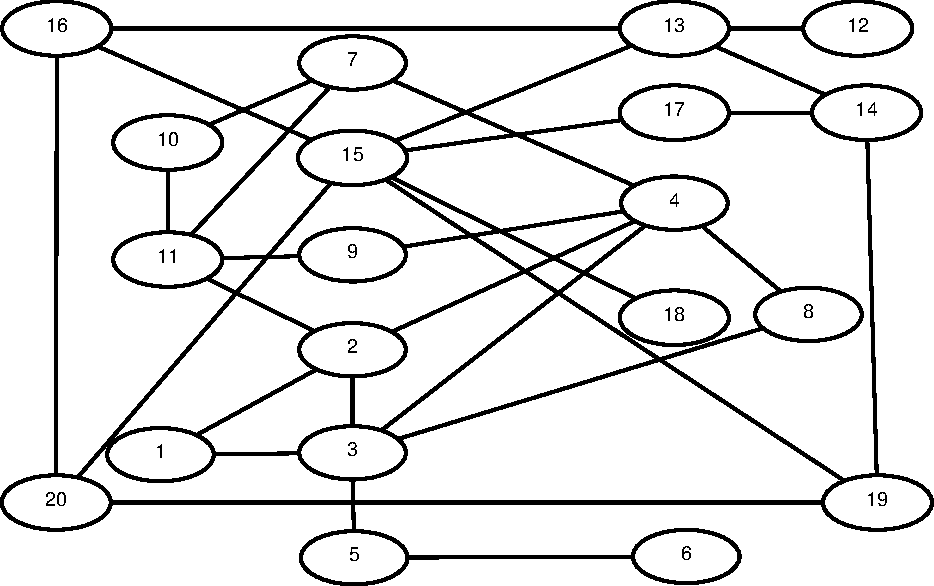
\includegraphics[width=0.75\linewidth]{images/buscaEmLargura00}
		\caption{}
		\label{fig:buscaemlargura00}
	\end{figure}
\end{frame}

\begin{frame}
	\frametitle{Algoritmos baseados em grafos}
	\framesubtitle{Árvores - Busca em largura - BFS}
	\setlength{\tabcolsep}{0.5em}
	\begin{tabular}{|c|c|c|c|c|c|c|c|c|c|c|c|c|c|c|c|c|c|c|c|c|}
		\hline
		\rule[0ex]{0pt}{0ex}&1&2&3&4&5&6&7&8&9&10&11&12&13&14&15&16&17&18&19&20 \\
		\hline
		\rule[0ex]{0pt}{0ex}V&0&0&0&0&0&0&0&0&0&0&0&0&0&0&0&0&0&0&0&0 \\
		\hline
		\rule[0ex]{0pt}{0ex}A&0&0&0&0&0&0&0&0&0&0&0&0&0&0&0&0&0&0&0&0 \\
		\hline
	\end{tabular}
	\par $F:\{\}$
	\begin{columns}
		\begin{column}{0.5\textwidth}
			\begin{figure}
				\centering
				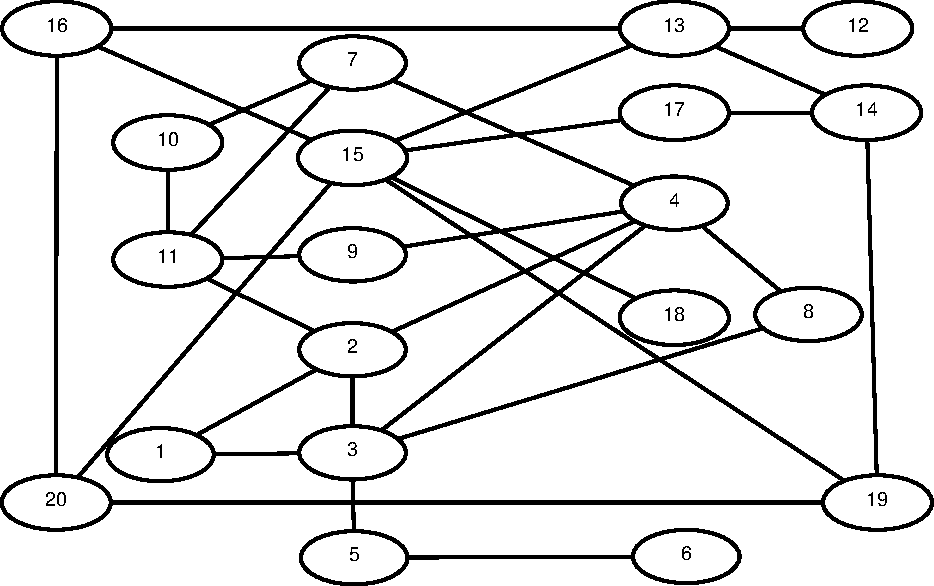
\includegraphics[width=\linewidth]{images/buscaEmLargura00}
				\caption{Grafo}
				\label{fig:buscaemlargura01}
			\end{figure}
		\end{column}
		\begin{column}{0.5\textwidth}
			\par Esse algoritmo começa com a criação de uma estrutura que marca quais vértices foram visitados ($V$), quais seus respectivos predecessores ($A$) e uma fila ($F$).
			\par Em seguida se escolhe de forma arbitrária um vértice por onde começar. Comecemos pelo vértice $2$, sendo assim, o mesmo entra na fila.
		\end{column}
	\end{columns}
\end{frame}

\begin{frame}
	\frametitle{Algoritmos baseados em grafos}
	\framesubtitle{Árvores - Busca em largura - BFS}
	\setlength{\tabcolsep}{0.5em}
	\begin{tabular}{|c|c|c|c|c|c|c|c|c|c|c|c|c|c|c|c|c|c|c|c|c|}
		\hline
		\rule[0ex]{0pt}{0ex}&1&2&3&4&5&6&7&8&9&10&11&12&13&14&15&16&17&18&19&20 \\
		\hline
		\rule[0ex]{0pt}{0ex}V&0&0&0&0&0&0&0&0&0&0&0&0&0&0&0&0&0&0&0&0 \\
		\hline
		\rule[0ex]{0pt}{0ex}A&2& &2&2&0&0&0&0&0&0&2&0&0&0&0&0&0&0&0&0 \\
		\hline
	\end{tabular}
	\par $F:\{\cancel{2},4,3,1,11\}$
	\begin{columns}
		\begin{column}{0.5\textwidth}
			\begin{figure}
				\centering
				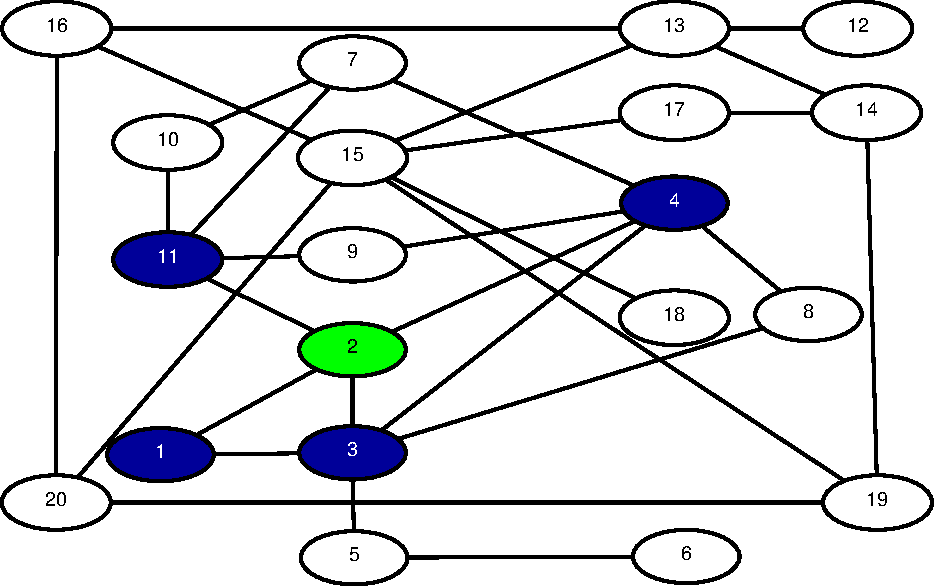
\includegraphics[width=\linewidth]{images/buscaEmLargura01}
				\caption{Grafo}
				\label{fig:buscaemlargura02}
			\end{figure}
		\end{column}
		\begin{column}{0.5\textwidth}
			\par Agora removemos o item mais antigo da fila e depois adicionamos na mesma seus vizinhos.
			\par Em seguida marcamos os nós visitados e indicamos seu predecessor (que é o $2$).
		\end{column}
	\end{columns}
\end{frame}

\begin{frame}
	\frametitle{Algoritmos baseados em grafos}
	\framesubtitle{Árvores - Busca em largura - BFS}
	\setlength{\tabcolsep}{0.5em}
	\begin{tabular}{|c|c|c|c|c|c|c|c|c|c|c|c|c|c|c|c|c|c|c|c|c|}
		\hline
		\rule[0ex]{0pt}{0ex}&1&2&3&4&5&6&7&8&9&10&11&12&13&14&15&16&17&18&19&20 \\
		\hline
		\rule[0ex]{0pt}{0ex}V&1&1&1&1&0&0&1&1&0&0&1&0&0&0&0&0&0&0&0&0 \\
		\hline
		\rule[0ex]{0pt}{0ex}A&2& &2&2&0&0&4&4&0&0&2&0&0&0&0&0&0&0&0&0 \\
		\hline
	\end{tabular}
	\par $F:\{\cancel{2},\cancel{4},3,1,11,7,8\}$
	\begin{columns}
		\begin{column}{0.5\textwidth}
			\begin{figure}
				\centering
				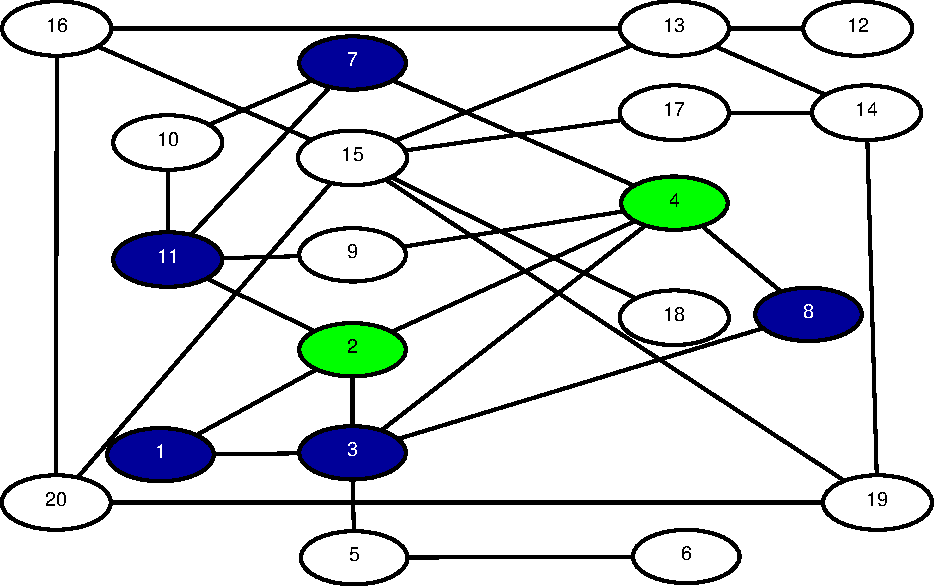
\includegraphics[width=\linewidth]{images/buscaEmLargura02}
				\caption{Grafo}
				\label{fig:buscaemlargura03}
			\end{figure}
		\end{column}
		\begin{column}{0.5\textwidth}
			\par Então \textbf{novamente} removemos o item mais antigo da fila e depois adicionamos na mesma seus vizinhos.
			\par Em seguida marcamos os nós visitados e indicamos seu predecessor (que é o $4$).
			\par Se faz isso \textbf{até que não exista item algum na fila}
		\end{column}
	\end{columns}
\end{frame}

\begin{frame}
	\frametitle{Algoritmos baseados em grafos}
	\framesubtitle{Árvores - Busca em largura - BFS}
	\setlength{\tabcolsep}{0.5em}
	\begin{tabular}{|c|c|c|c|c|c|c|c|c|c|c|c|c|c|c|c|c|c|c|c|c|}
		\hline
		\rule[0ex]{0pt}{0ex}&1&2&3&4&5&6&7&8&9&10&11&12&13&14&15&16&17&18&19&20 \\
		\hline
		\rule[0ex]{0pt}{0ex}V&1&1&1&1&1&0&1&1&0&0&1&0&0&0&0&0&0&0&0&0 \\
		\hline
		\rule[0ex]{0pt}{0ex}A&2& &2&2&3&0&4&4&0&0&2&0&0&0&0&0&0&0&0&0 \\
		\hline
	\end{tabular}
	\begin{columns}
		\begin{column}{0.5\textwidth}
			\only<1>{
				\par $F:\{\cancel{2},\cancel{4},\cancel{3},1,11,7,8,5\}$
				\begin{figure}
					\centering
					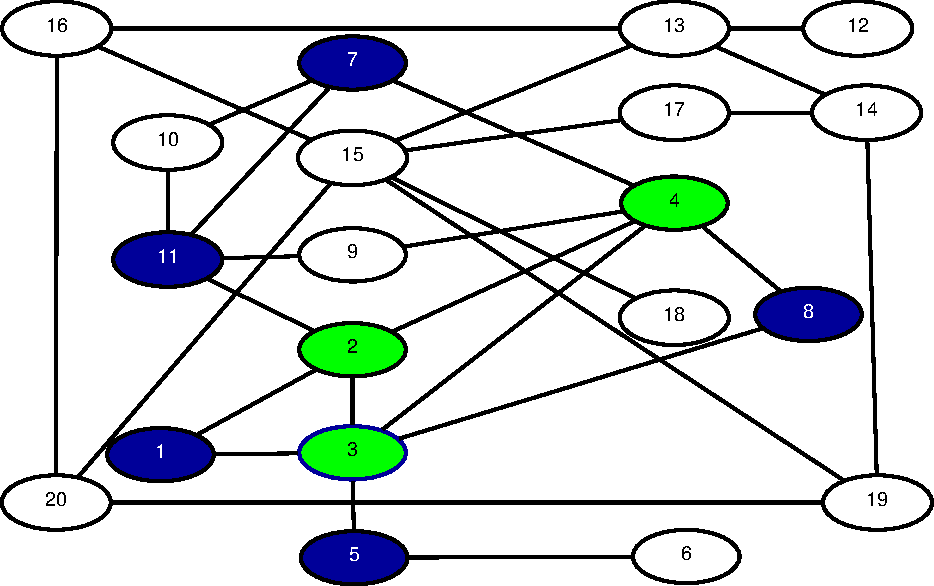
\includegraphics[width=\linewidth]{images/buscaEmLargura03}
					\caption{Grafo}
					\label{fig:buscaemlargura04}
				\end{figure}
			}
			\only<2>{
				\par $F:\{\cancel{2},\cancel{4},\cancel{3},\cancel{1},11,7,8,5\}$
				\begin{figure}
					\centering
					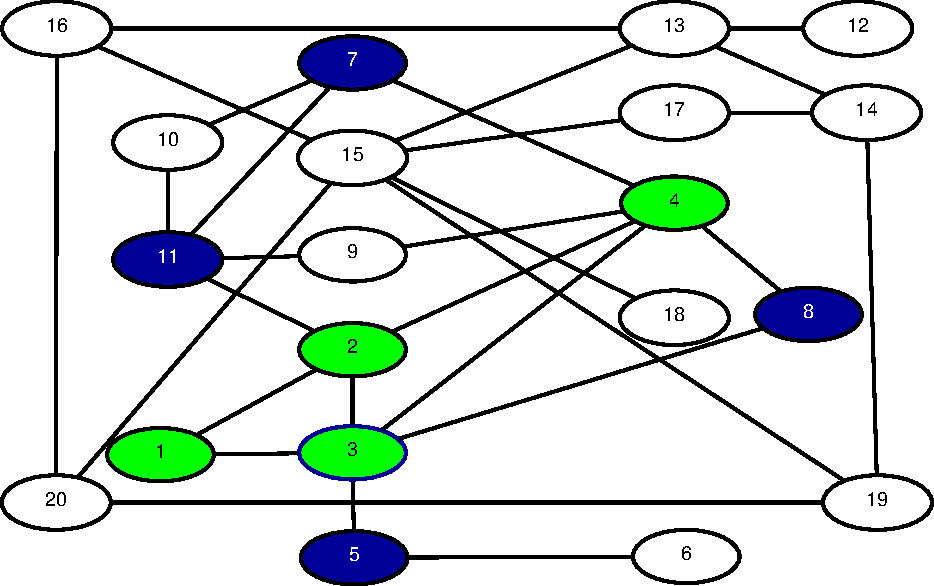
\includegraphics[width=\linewidth]{images/buscaEmLargura04}
					\caption{Grafo}
					\label{fig:buscaemlargura05}
				\end{figure}
			}
		\end{column}
		\begin{column}{0.5\textwidth}

		\end{column}
	\end{columns}
\end{frame}

\begin{frame}
	\frametitle{Algoritmos baseados em grafos}
	\framesubtitle{Árvores - Busca em largura - BFS}
	\setlength{\tabcolsep}{0.5em}
	\begin{tabular}{|c|c|c|c|c|c|c|c|c|c|c|c|c|c|c|c|c|c|c|c|c|}
		\hline
		\rule[0ex]{0pt}{0ex}&1&2&3&4&5&6&7&8&9&10&11&12&13&14&15&16&17&18&19&20 \\
		\hline
		\rule[0ex]{0pt}{0ex}V&1&1&1&1&1&0&1&1&1&1&1&0&0&0&0&0&0&0&0&0 \\
		\hline
		\rule[0ex]{0pt}{0ex}A&2& &2&2&3&0&4&4&11&11&2&0&0&0&0&0&0&0&0&0 \\
		\hline
	\end{tabular}
	\begin{columns}
		\begin{column}{0.5\textwidth}
			\only<1>{
				\par $F:\{\cancel{2},\cancel{4},\cancel{3},\cancel{1},\cancel{11},\cancel{7},8,5,10,9\}$
				\begin{figure}
					\centering
					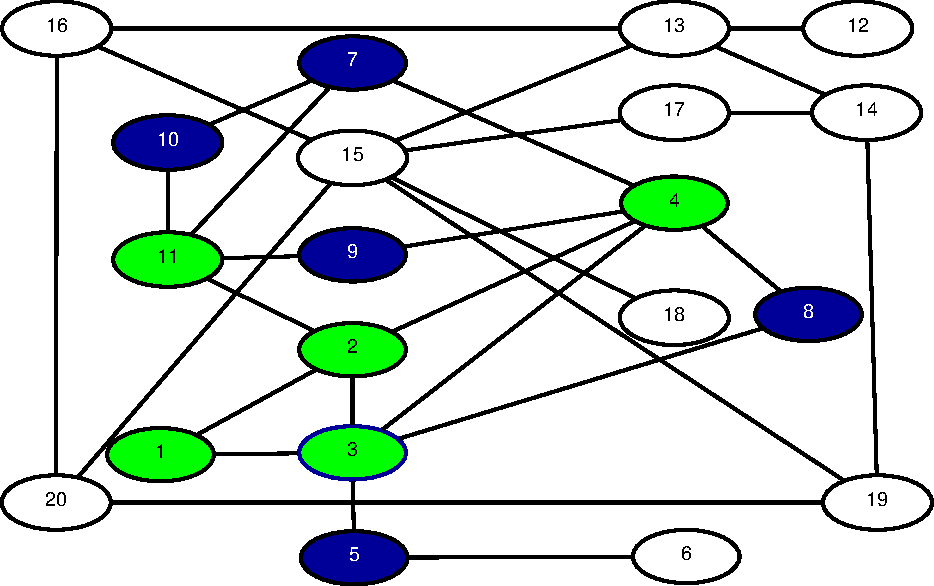
\includegraphics[width=\linewidth]{images/buscaEmLargura05}
					\caption{Grafo}
					\label{fig:buscaemlargura06}
				\end{figure}
			}
			\only<2>{
				\par $F:\{\cancel{2},\cancel{4},\cancel{3},\cancel{1},\cancel{11},\cancel{7},8,5,10,9\}$
				\begin{figure}
					\centering
					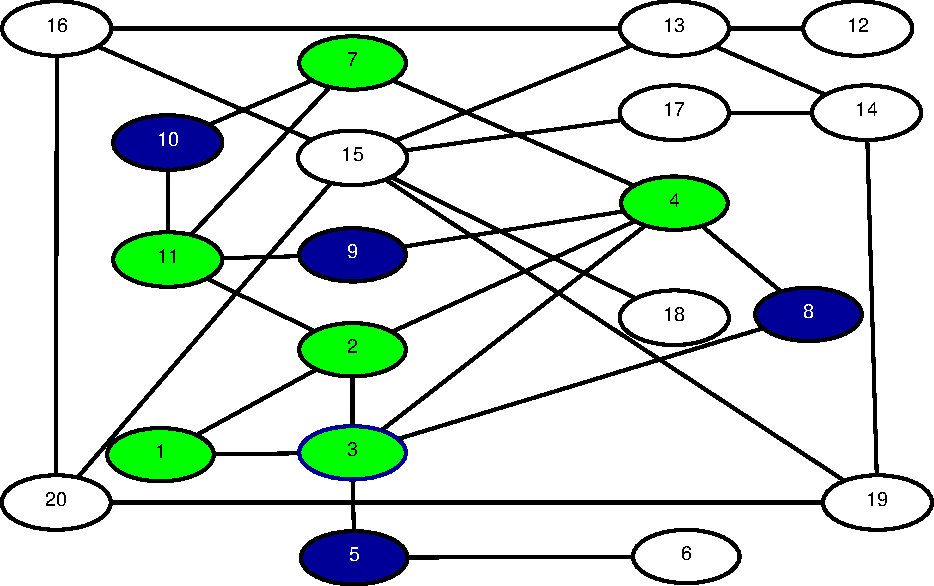
\includegraphics[width=\linewidth]{images/buscaEmLargura06}
					\caption{Grafo}
					\label{fig:buscaemlargura07}
				\end{figure}
			}
		\end{column}
		\begin{column}{0.5\textwidth}

		\end{column}
	\end{columns}
\end{frame}

\begin{frame}
	\frametitle{Algoritmos baseados em grafos}
	\framesubtitle{Árvores - Busca em largura - BFS}
	\setlength{\tabcolsep}{0.5em}
	\begin{tabular}{|c|c|c|c|c|c|c|c|c|c|c|c|c|c|c|c|c|c|c|c|c|}
		\hline
		\rule[0ex]{0pt}{0ex}&1&2&3&4&5&6&7&8&9&10&11&12&13&14&15&16&17&18&19&20 \\
		\hline
		\rule[0ex]{0pt}{0ex}V&1&1&1&1&1&1&1&1&1&1&1&0&0&0&0&0&0&0&0&0 \\
		\hline
		\rule[0ex]{0pt}{0ex}A&2& &2&2&3&5&4&4&11&11&2&0&0&0&0&0&0&0&0&0 \\
		\hline
	\end{tabular}
	\begin{columns}
		\begin{column}{0.5\textwidth}
			\only<1>{
				\par $F:\{\cancel{2},\cancel{4},\cancel{3},\cancel{1},\cancel{11},\cancel{7},\cancel{8},5,10,9\}$
				\begin{figure}
					\centering
					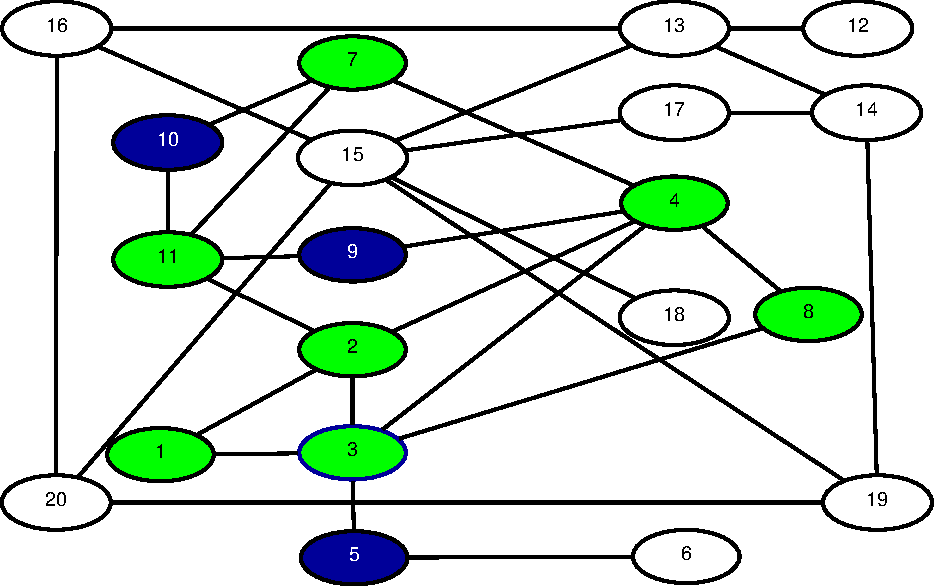
\includegraphics[width=\linewidth]{images/buscaEmLargura07}
					\caption{Grafo}
					\label{fig:buscaemlargura08}
				\end{figure}
			}
			\only<2>{
				\par $F:\{\cancel{2},\cancel{4},\cancel{3},\cancel{1},\cancel{11},\cancel{7},\cancel{8},\cancel{5},10,9,6\}$
				\begin{figure}
					\centering
					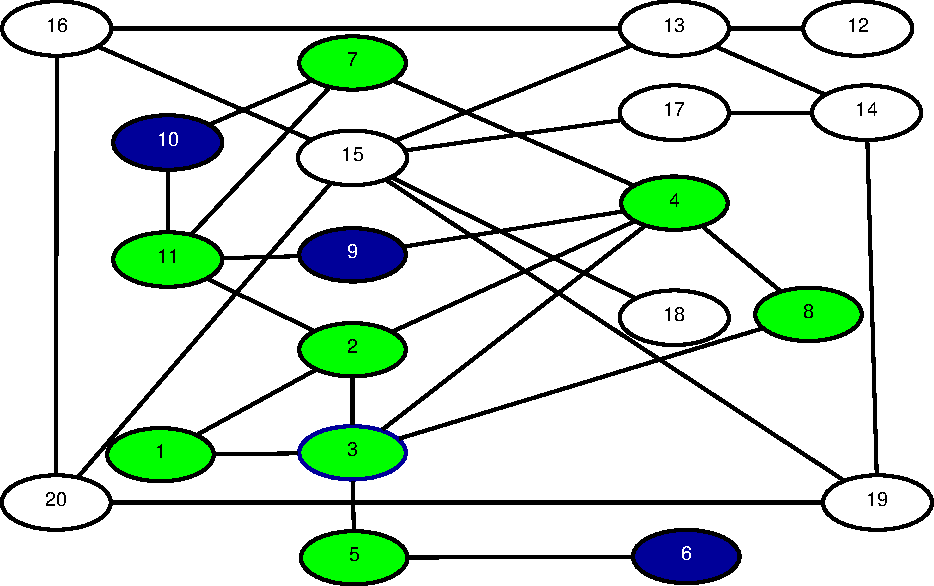
\includegraphics[width=\linewidth]{images/buscaEmLargura08}
					\caption{Grafo}
					\label{fig:buscaemlargura09}
				\end{figure}
			}
		\end{column}
		\begin{column}{0.5\textwidth}

		\end{column}
	\end{columns}
\end{frame}

\begin{frame}
	\frametitle{Algoritmos baseados em grafos}
	\framesubtitle{Árvores - Busca em largura - BFS}
	\setlength{\tabcolsep}{0.5em}
	\begin{tabular}{|c|c|c|c|c|c|c|c|c|c|c|c|c|c|c|c|c|c|c|c|c|}
		\hline
		\rule[0ex]{0pt}{0ex}&1&2&3&4&5&6&7&8&9&10&11&12&13&14&15&16&17&18&19&20 \\
		\hline
		\rule[0ex]{0pt}{0ex}V&1&1&1&1&1&1&1&1&1&1&1&0&0&0&0&0&0&0&0&0 \\
		\hline
		\rule[0ex]{0pt}{0ex}A&2& &2&2&3&5&4&4&11&11&2&0&0&0&0&0&0&0&0&0 \\
		\hline
	\end{tabular}
	\begin{columns}
		\begin{column}{0.5\textwidth}
			\only<1>{
				\par $F:\{\cancel{2},\cancel{4},\cancel{3},\cancel{1},\cancel{11},\cancel{7},\cancel{8},\cancel{5},\cancel{10},9,6\}$
				\begin{figure}
					\centering
					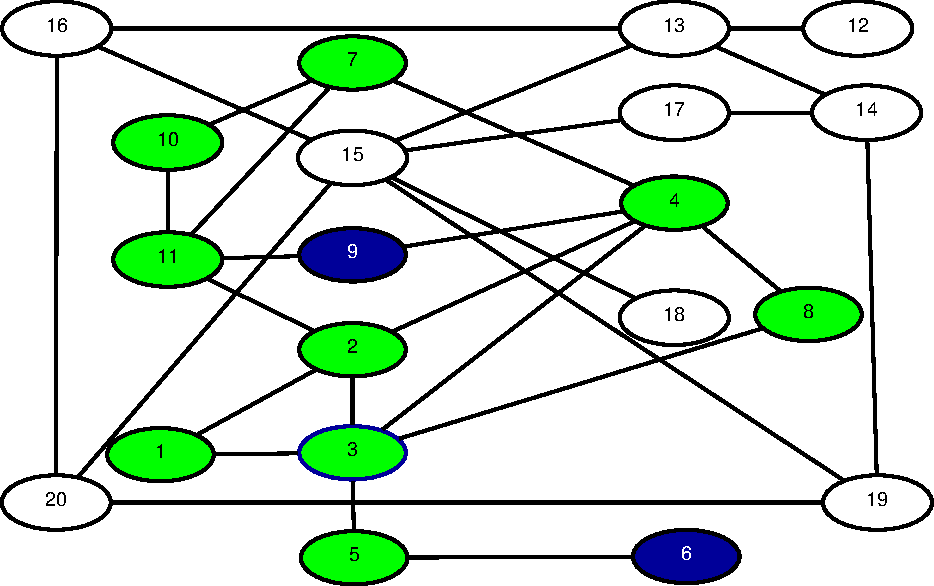
\includegraphics[width=\linewidth]{images/buscaEmLargura09}
					\caption{Grafo}
					\label{fig:buscaemlargura10}
				\end{figure}
			}
			\only<2>{
				\par
	$F:\{\cancel{2},\cancel{4},\cancel{3},\cancel{1},\cancel{11},\cancel{7},\cancel{8},\cancel{5},\cancel{10},\cancel{9},6\}$
				\begin{figure}
					\centering
					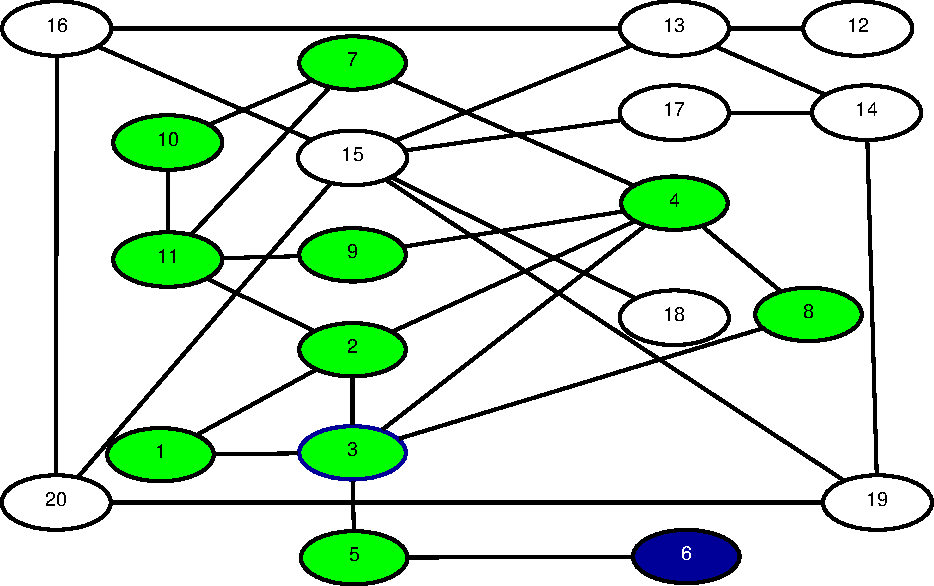
\includegraphics[width=\linewidth]{images/buscaEmLargura10}
					\caption{Grafo}
					\label{fig:buscaemlargura11}
				\end{figure}
			}
		\end{column}
		\begin{column}{0.5\textwidth}

		\end{column}
	\end{columns}
\end{frame}

\begin{frame}
	\frametitle{Algoritmos baseados em grafos}
	\framesubtitle{Árvores - Busca em largura - BFS}
	\setlength{\tabcolsep}{0.5em}
	\begin{tabular}{|c|c|c|c|c|c|c|c|c|c|c|c|c|c|c|c|c|c|c|c|c|}
		\hline
		\rule[0ex]{0pt}{0ex}&1&2&3&4&5&6&7&8&9&10&11&12&13&14&15&16&17&18&19&20 \\
		\hline
		\rule[0ex]{0pt}{0ex}V&1&1&1&1&1&1&1&1&1&1&1&0&0&0&0&0&0&0&0&0 \\
		\hline
		\rule[0ex]{0pt}{0ex}A&2& &2&2&3&5&4&4&11&11&2&0&0&0&0&0&0&0&0&0 \\
		\hline
	\end{tabular}
	\begin{columns}
		\begin{column}{0.5\textwidth}
			\par $F:\{\cancel{2},\cancel{4},\cancel{3},\cancel{1},\cancel{11},\cancel{7},\cancel{8},\cancel{5},\cancel{10},\cancel{9},\cancel{6}\}$
			\begin{figure}
				\centering
				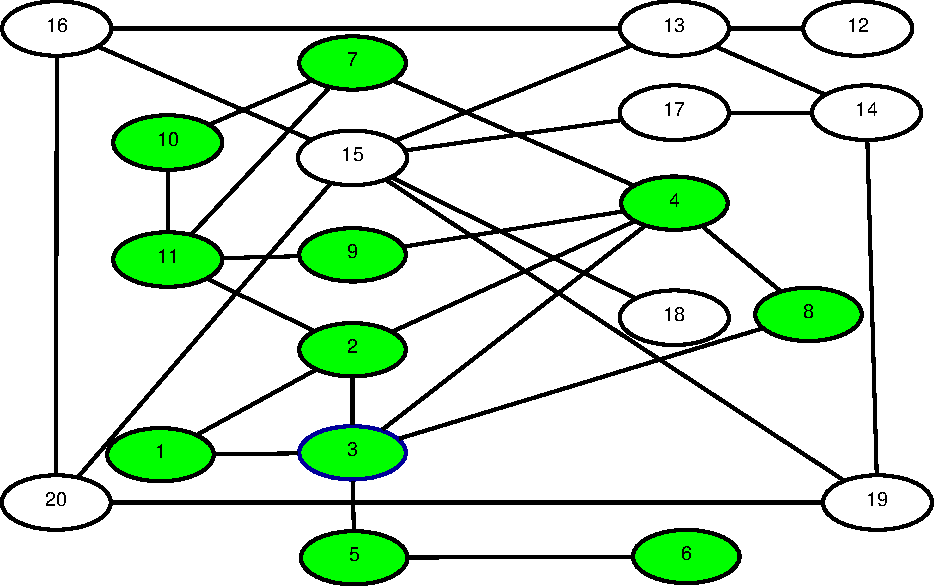
\includegraphics[width=\linewidth]{images/buscaEmLargura11}
				\caption{Grafo}
				\label{fig:buscaemlargura12}
			\end{figure}
		\end{column}
		\pause
		\begin{column}{0.5\textwidth}
			\par Fim!
			\par Perceba que uma parte do grafo ficou de fora, ou seja, este é um grafo desconexo, mesmo que dentro dele existam \textbf{dois} grafos conexos.
		\end{column}
	\end{columns}
\end{frame}

\begin{frame}
	\frametitle{Algoritmos baseados em grafos}
	\framesubtitle{Árvores - Busca em largura - BFS}
	\begin{columns}
		\begin{column}{0.5\textwidth}
			\begin{figure}
				\centering
				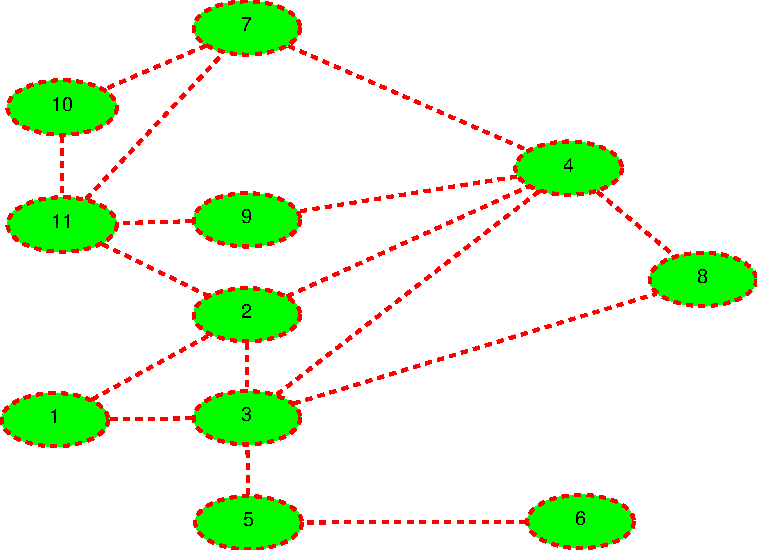
\includegraphics[width=\linewidth]{images/buscaEmLargura12}
				\caption{Subgrafo 01}
				\label{fig:buscaemlargura13}
			\end{figure}
		\end{column}
		\begin{column}{0.5\textwidth}
			\begin{figure}
				\centering
				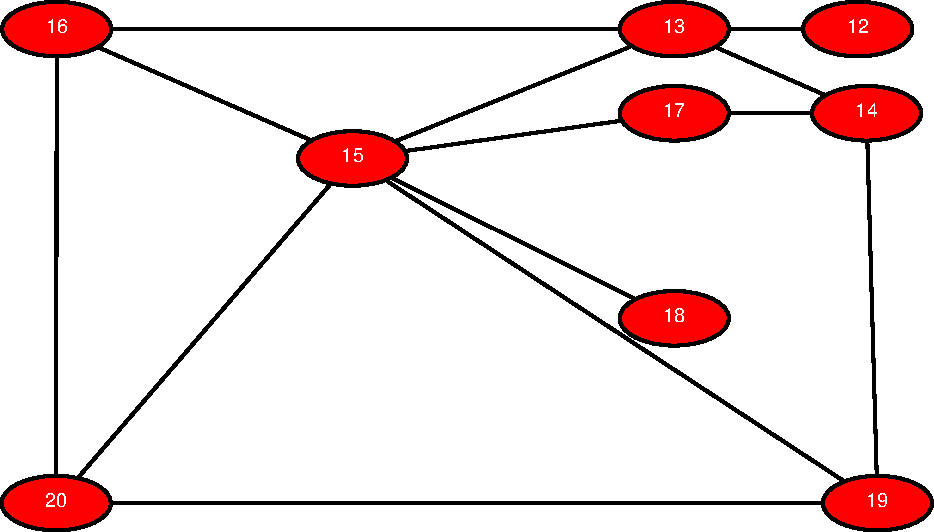
\includegraphics[width=\linewidth]{images/buscaEmLargura13}
				\caption{Subgrafo 02}
				\label{fig:buscaemlargura14}
			\end{figure}
		\end{column}
	\end{columns}
\end{frame}

\begin{frame}
	\frametitle{Algoritmos de busca em grafos}
	\framesubtitle{Busca em largura - Exercício 06}
	\par \textbf{Implemente} a busca em largura e resolva o problema demonstrado nos slides anteriores. Qual o tempo assintótico de execução?
	\par A partir da raiz da árvore criada é possível achar o menor caminho até um outro vértice qualquer? Como?
\end{frame}

\begin{frame}[allowframebreaks]
	\frametitle{Algoritmos de busca em grafos}
	\framesubtitle{Árvores - Exercício 06}
	\par \textbf{Resposta:}
	\par O tempo de execução depende da implementação (matriz ou lista de adjacências).
	\par Para listas: $\Theta(1) + \Theta(1) + \Theta(1) + \Theta(V(G)) + O(A(G)) =O(V(G)+A(G)) $
	\par Para Matriz: $\Theta(1) + \Theta(1) + \Theta(1) + \Theta(V)G))*\Theta(V(G)) = \Theta(V(G)^2)$
	\lstinputlisting[language=C++]{../codigo/buscaEmLargura.cpp}
\end{frame}

\begin{frame}
	\frametitle{Algoritmos de busca em grafos}
	\framesubtitle{Busca em profundidade - DSF}
	\par Ao contrário do algoritmo anterior essa busca se dá pelo \textbf{vértice descoberto mais recentemente} até que o mesmo não tenha mais vizinhos. Descobertos todos os vizinhos a busca se volta para o vértice anterior. Esse tipo de busca monta \textbf{florestas} a partir dos grafos dados.
	
	\par Os passos do algoritmo são os seguintes:
	\begin{enumerate}
		\item escolha um vértice não vistado, se não houver \textbf{pare} \label{enum:nvisit}
		\item marque-o como visitado
		\item \textbf{empilhe} ele
		\item escolha um vizinho, senão houver volte para \ref{enum:nvisit} \label{enum:vizinho}
		\item marque-o como visitado
		\item se o vizinho tiver vizinhos \textbf{empilhe ele} senão desempilhe
		\item Volte ao item \ref{enum:vizinho}
	\end{enumerate}
\end{frame}

\begin{frame}
	\frametitle{Algoritmos de busca em grafos}
	\framesubtitle{Busca em profundidade - Exercício 07}
	\par \textbf{Implemente} a busca em profundidade alterando o BFS
	\par \alert{Alerta de spoiler} o tempo de execução é $O(V(G)+A(G))$! Porque?
\end{frame}

\begin{frame}
	\frametitle{Algoritmos de busca em grafos}
	\framesubtitle{Árvores binárias}
	\par Uma \textbf{árvore binária completa} tem todos os níveis completamente cheios, exceto possivelmente o último, sendo que todos os nós no último nível estão tanto à esquerda quanto possível. Já uma \textbf{cheia} tem cada um do nós com 2 ou 0 ramos. 
	\begin{figure}
		\centering
		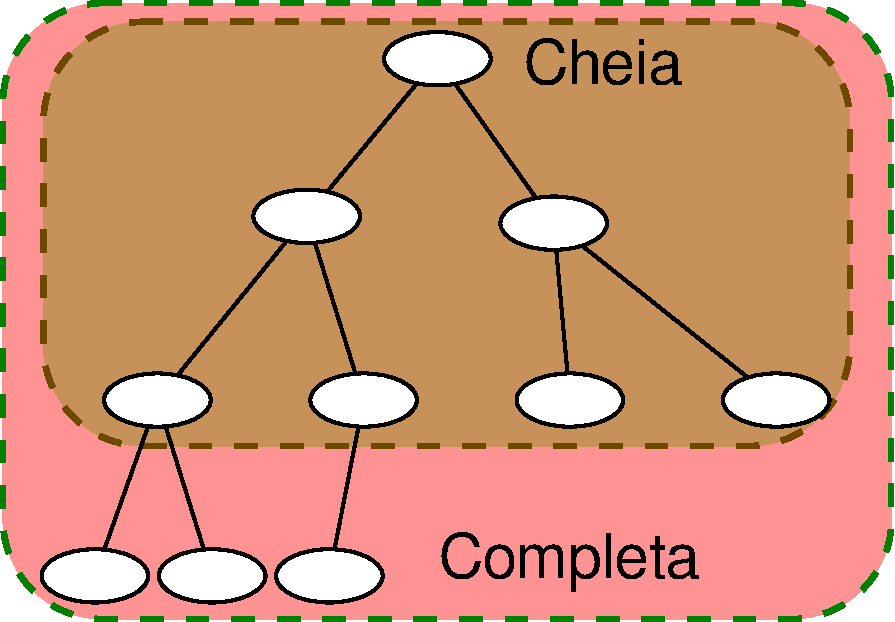
\includegraphics[width=0.5\linewidth]{images/arvoreBinaria}
		\caption{Árvore binária}
		\label{fig:arvorebinaria}
	\end{figure}
\end{frame}

\begin{frame}
	\frametitle{Algoritmos de busca em grafos}
	\framesubtitle{ABB - Árvore de busca binária}
	\par Além de cada nó ter, no máximo, dois ramos os nós filhos a esquerda devem ser menores que sua raiz e os da direita devem ser maiores.
	\par Se não houver um cuidado em balancear a árvore ela pode degenerar em uma lista.
	\begin{figure}
		\centering
		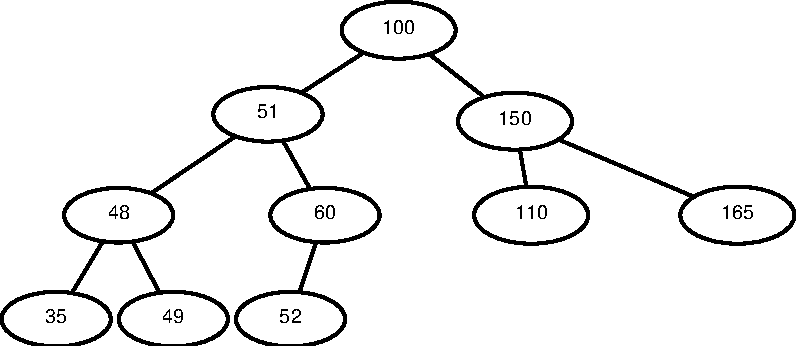
\includegraphics[width=0.6\linewidth]{images/arvoreBinariaBusca}
		\caption{Árvore binária de busca}
		\label{fig:arvorebinariabusca}
	\end{figure}
\end{frame}

\begin{frame}
	\frametitle{Algoritmos de busca em grafos}
	\framesubtitle{AVL - Árvore binária de busca balanceada}
	\par Cada nó tem, no máximo, dois ramos ou folhas.
	\par \textbf{Não é} degenerada, ou seja, não balanceada.
	\par Dada um árvore binária a diferença de altura entre os ramos à esquerda e a direita vai ser \textbf{no máximo} 1.
	\par A AVLs tem nós, se diz que um nó é \textbf{regulado} quando a diferença entre as alturas de seus ramos é \textbf{no máximo} 1.
	\par Quando todos os nós da árvore estão regulados então temos uma AVL.
	\begin{columns}
		\begin{column}{0.33\textwidth}
			\begin{figure}
				\centering
				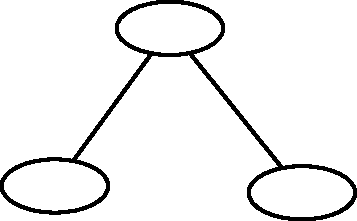
\includegraphics[width=.7\linewidth]{images/AVL0}
				\caption{AVL}
				\label{fig:avl0}
			\end{figure}
		\end{column}
		\begin{column}{0.33\textwidth}
			\begin{figure}
				\centering
				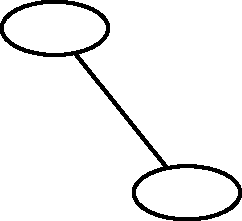
\includegraphics[width=.4\linewidth]{images/AVL1}
				\caption{AVL}
				\label{fig:avl1}
			\end{figure}
		\end{column}
		\begin{column}{0.33\textwidth}
			\begin{figure}
				\centering
				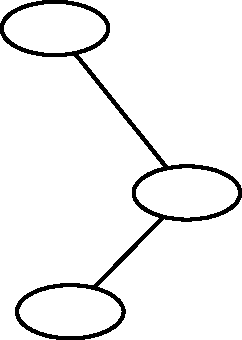
\includegraphics[width=.3\linewidth]{images/naoAVL}
				\caption{Não AVL}
				\label{fig:naoavl}
			\end{figure}
		\end{column}
	\end{columns}
\end{frame}

\begin{frame}
	\frametitle{Algoritmos de busca em grafos}
	\framesubtitle{AVL - Árvore de busca balanceada - Percurso em ordem}
	\par É uma forma de realizar um \textbf{percurso} na árvore binária. Um percurso é uma forma \textbf{sistemática} de percorrer os nós de uma árvore.
	\par No percuso em ordem o último elemento a ser exibido está sempre ao lado direito da raiz das árvores e sub-árvores e quando um elemento \textbf{não tem} filho a esquerda \textbf{que não foi mostrado} ele também é mostrado
	
	\only<1>{
		\begin{figure}
			\centering
			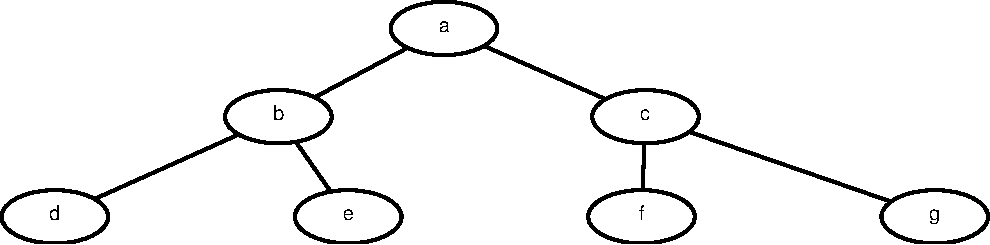
\includegraphics[width=0.7\linewidth]{images/arvoreBinaria2}
			\caption{Árvore binária}
			\label{fig:arvorebinaria3}
		\end{figure}
	}
	\only<2>{
		\par $G = \{d\}$
		\begin{figure}
			\centering
			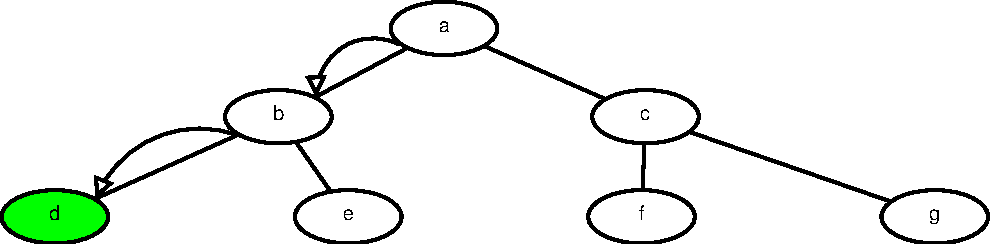
\includegraphics[width=0.7\linewidth]{images/emordem0}
			\caption{Em ordem}
			\label{fig:emordem0}
		\end{figure}
	}
	\only<3>{
		\par $G = \{d,b\}$
		\begin{figure}
			\centering
			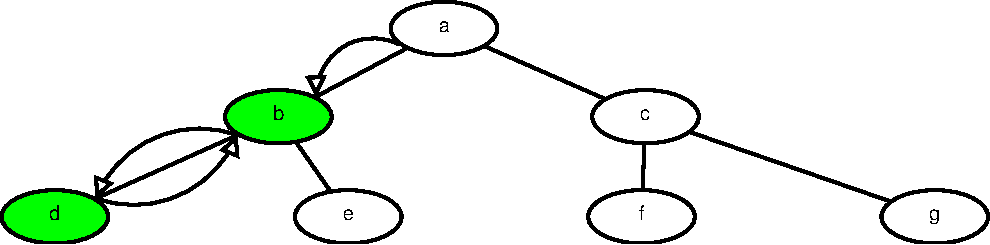
\includegraphics[width=0.7\linewidth]{images/emordem1}
			\caption{Em ordem}
			\label{fig:emordem1}
		\end{figure}
	}	
	\only<4>{
		\par $G = \{d,b,e\}$
		\begin{figure}
			\centering
			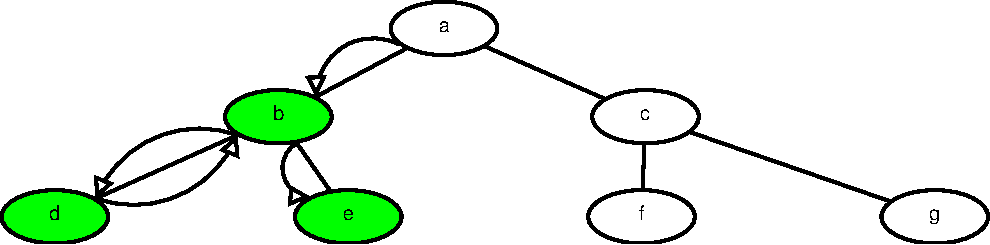
\includegraphics[width=0.7\linewidth]{images/emordem2}
			\caption{Em ordem}
			\label{fig:emordem2}
		\end{figure}
	}
	\only<5>{
		\par $G = \{d,b,e,a\}$
		\begin{figure}
			\centering
			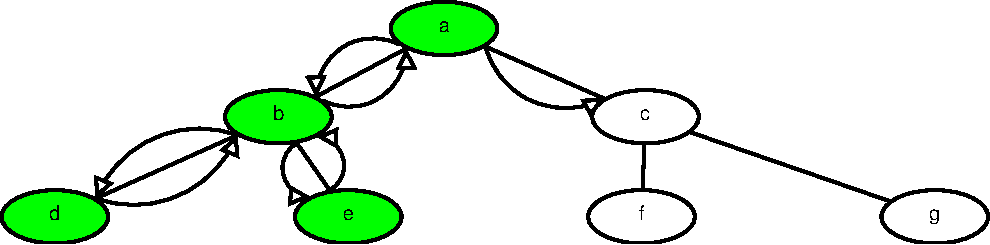
\includegraphics[width=0.7\linewidth]{images/emordem3}
			\caption{Em ordem}
			\label{fig:emordem3}
		\end{figure}
	}
	\only<6>{
		\par $G = \{d,b,e,a,f\}$
		\begin{figure}
			\centering
			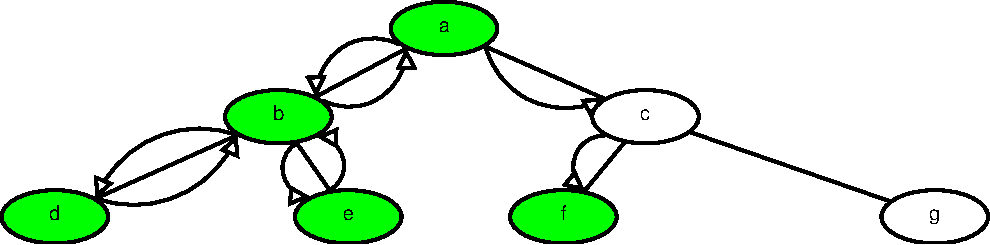
\includegraphics[width=0.7\linewidth]{images/emordem4}
			\caption{Em ordem}
			\label{fig:emordem4}
		\end{figure}
	}
	\only<7>{
		\par $G = \{d,b,e,a,f,c\}$
		\begin{figure}
			\centering
			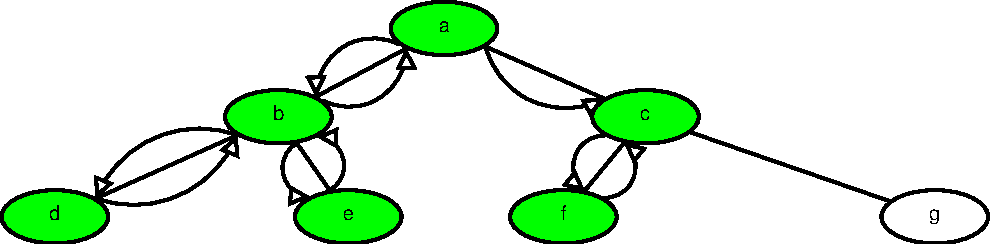
\includegraphics[width=0.7\linewidth]{images/emordem5}
			\caption{Em ordem}
			\label{fig:emordem5}
		\end{figure}
	}
	\only<8>{
		\par $G = \{d,b,e,a,f,c,g\}$
		\begin{figure}
			\centering
			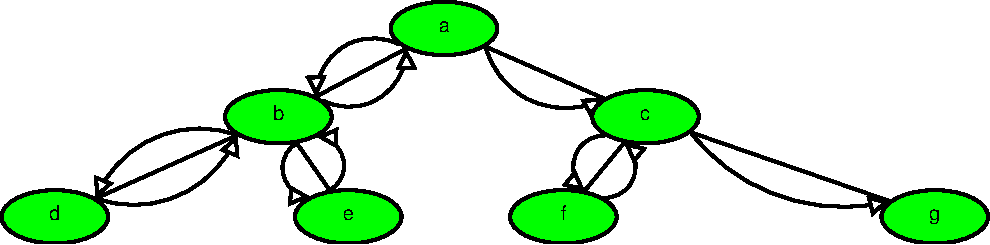
\includegraphics[width=0.7\linewidth]{images/emordem6}
			\caption{Em ordem}
			\label{fig:emordem6}
		\end{figure}
	}
\end{frame}

\begin{frame}
	\frametitle{Algoritmos de busca em grafos}
	\framesubtitle{AVL - Árvore de busca balanceada - Percurso pós-ordem}
	\par No percuso pós-ordem a raiz da árvore será o último nós a ser visitado, sendo assim, considerando que sub-árvores também tem suas raízes as mesmas terão, da mesma forma, suas raízes visitadas por último. Notou o padrão recursivo?
	
	\only<1>{
	\begin{figure}
		\centering
		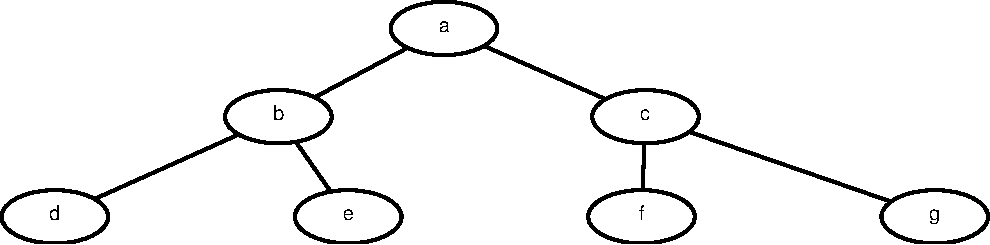
\includegraphics[width=0.7\linewidth]{images/arvoreBinaria2}
		\caption{Árvore binária}
		\label{fig:arvorebinaria2}
	\end{figure}
	}
	\only<2>{
	\par $G = \{\emptyset\}$
	\begin{figure}
		\centering
		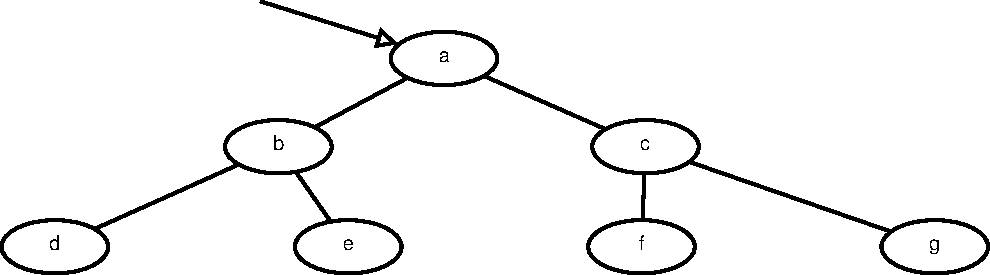
\includegraphics[width=0.7\linewidth]{images/posordem0}
		\caption{Pós-ordem}
		\label{fig:posordem0}
	\end{figure}
	}
	\only<3>{
	\par $G = \{\emptyset\}$
	\begin{figure}
		\centering
		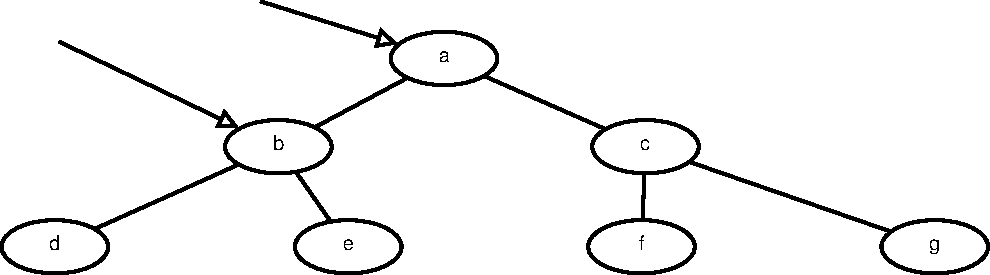
\includegraphics[width=0.7\linewidth]{images/posordem1}
		\caption{Pós-ordem}
		\label{fig:posordem1}
	\end{figure}
	}	
	\only<4>{
	\par $G = \{d\}$
	\begin{figure}
		\centering
		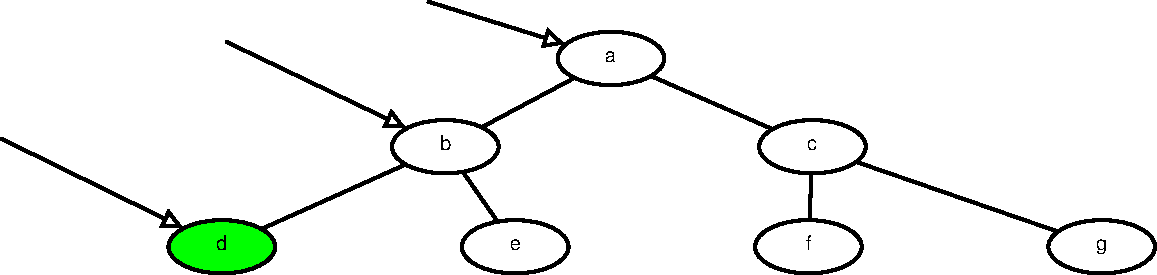
\includegraphics[width=0.7\linewidth]{images/posordem2}
		\caption{Pós-ordem}
		\label{fig:posordem2}
	\end{figure}
	}
	\only<5>{
	\par $G = \{d,e\}$
	\begin{figure}
		\centering
		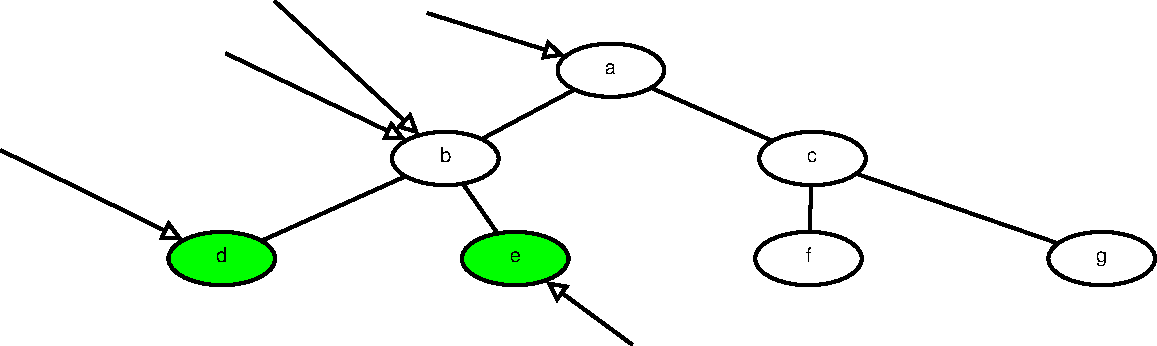
\includegraphics[width=0.7\linewidth]{images/posordem3}
		\caption{Pós-ordem}
		\label{fig:posordem3}
	\end{figure}
	}
	\only<6>{
	\par $G = \{d,e,b\}$
	\begin{figure}
		\centering
		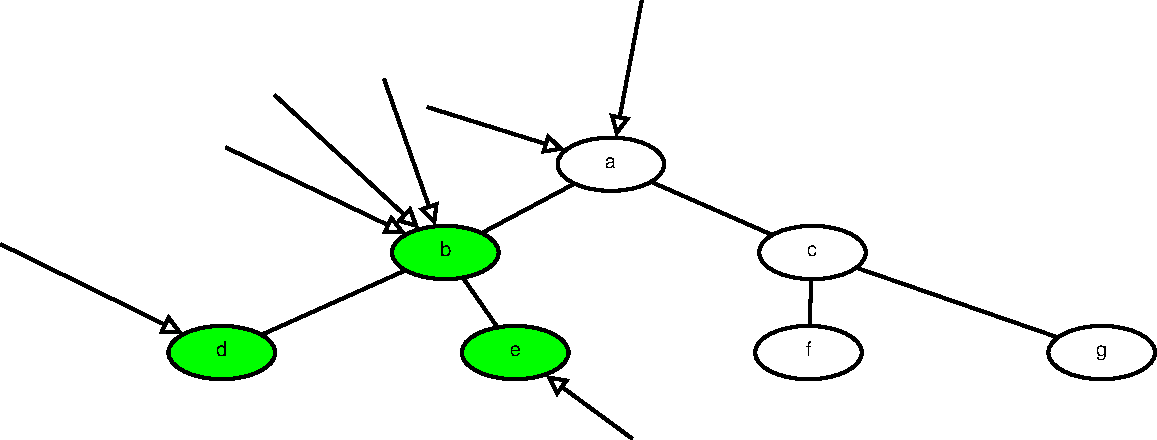
\includegraphics[width=0.7\linewidth]{images/posordem4}
		\caption{Pós-ordem}
		\label{fig:posordem4}
	\end{figure}
	}
	\only<7>{
	\par $G = \{d,e,b\}$
	\begin{figure}
		\centering
		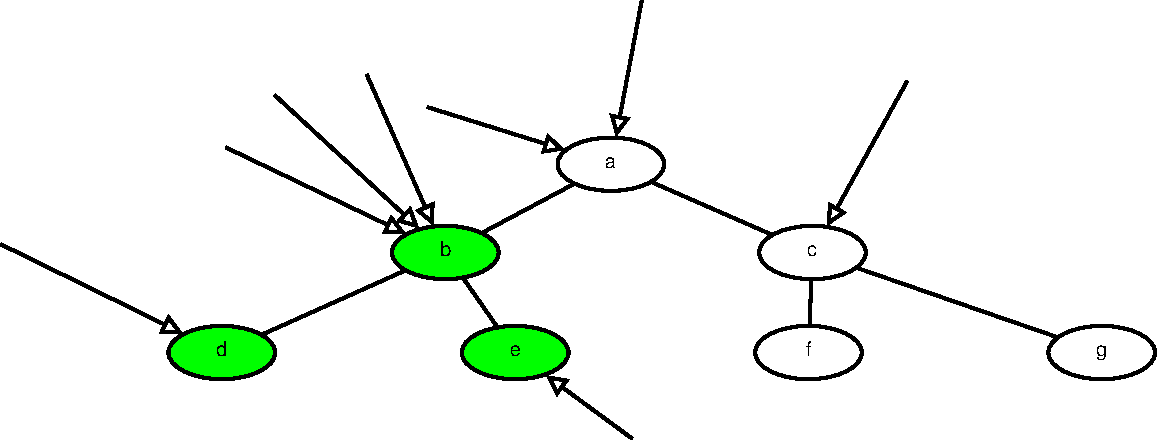
\includegraphics[width=0.7\linewidth]{images/posordem5}
		\caption{Pós-ordem}
		\label{fig:posordem5}
	\end{figure}
	}
	\only<8>{
	\par $G = \{d,e,b,f\}$
	\begin{figure}
		\centering
		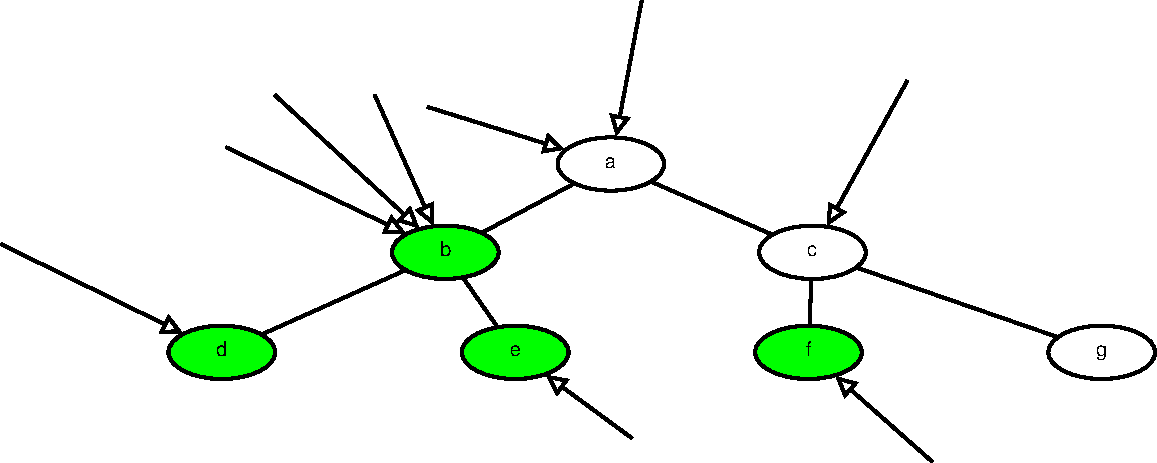
\includegraphics[width=0.7\linewidth]{images/posordem6}
		\caption{Pós-ordem}
		\label{fig:posordem6}
	\end{figure}
	}
	\only<9>{
	\par $G = \{d,e,b,f,g\}$
	\begin{figure}
		\centering
		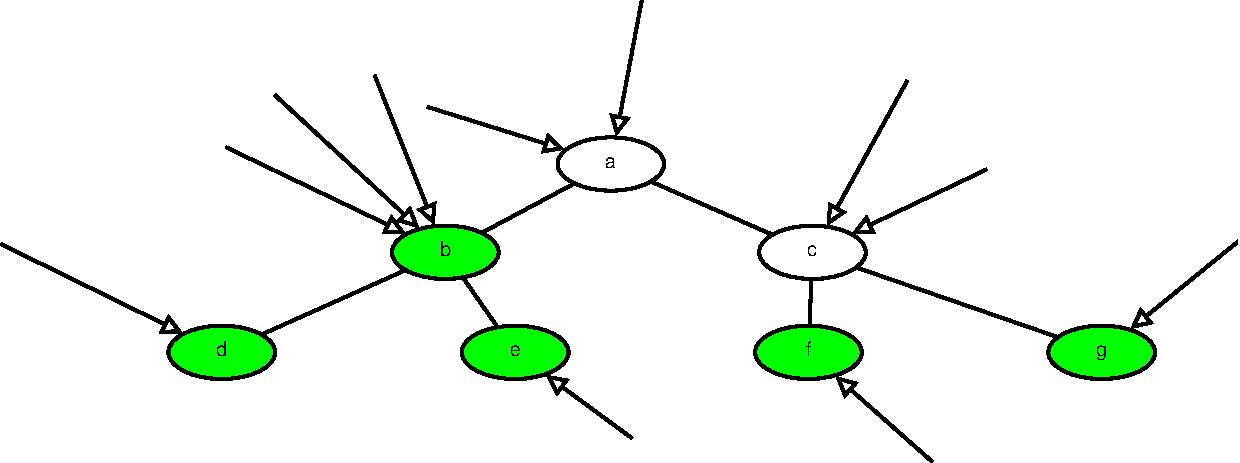
\includegraphics[width=0.7\linewidth]{images/posordem7}
		\caption{Pós-ordem}
		\label{fig:posordem7}
	\end{figure}
	}
	\only<10>{
	\par $G = \{d,e,b,f,g,c\}$
	\begin{figure}
		\centering
		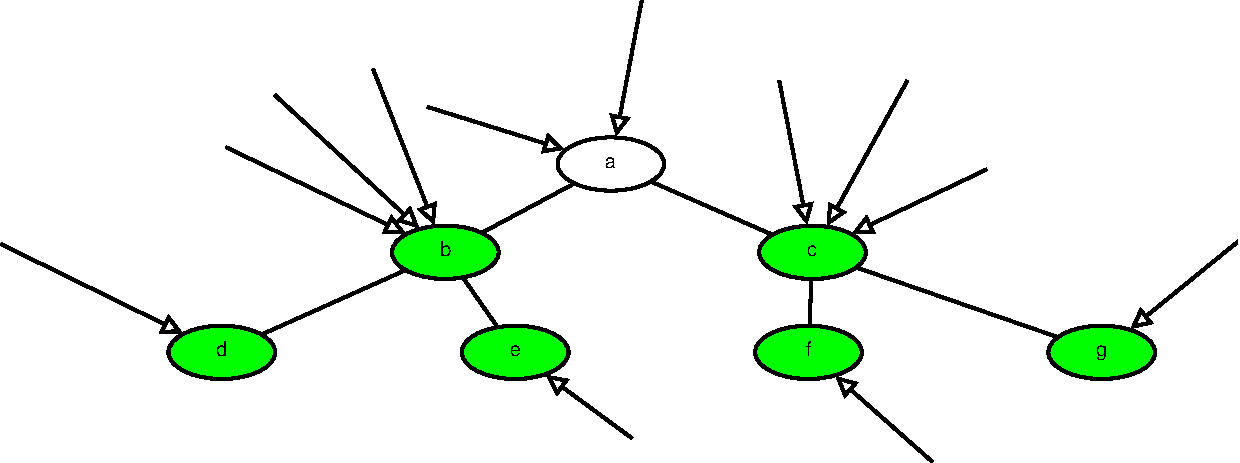
\includegraphics[width=0.7\linewidth]{images/posordem8}
		\caption{Pós-ordem}
		\label{fig:posordem8}
	\end{figure}
	}
	\only<11>{
	\par $G = \{d,e,b,f,g,c,a\}$
	\begin{figure}
		\centering
		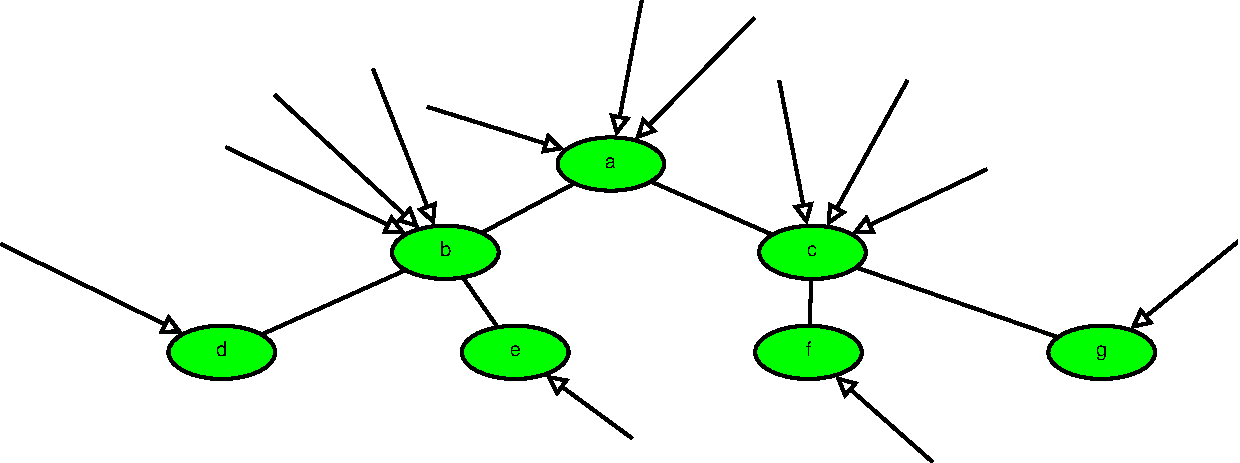
\includegraphics[width=0.7\linewidth]{images/posordem9}
		\caption{Pós-ordem}
		\label{fig:posordem9}
	\end{figure}
	}
\end{frame}

\begin{frame}
	\frametitle{Algoritmos de busca em grafos}
	\framesubtitle{AVL - Árvore de busca balanceada - Percurso pré-ordem - Exercício0}
	
	\par No percurso em pré-ordem sempre que a raíz de uma árvore ou sub-árvore é visitado o mesmo é exibido para em seguida se visitar o próximo nó a esquerda \textbf{até que não haja mais nós esquerdos}, depois disso se exibe os nós a direita.

	\par \textbf{Desenhe} o percurso da árvore binária em pré-ordem.
	\pause
	\par \textbf{Resposta:} $G = \{a,b,d,e,c,f,g\}$
	\begin{figure}
		\centering
		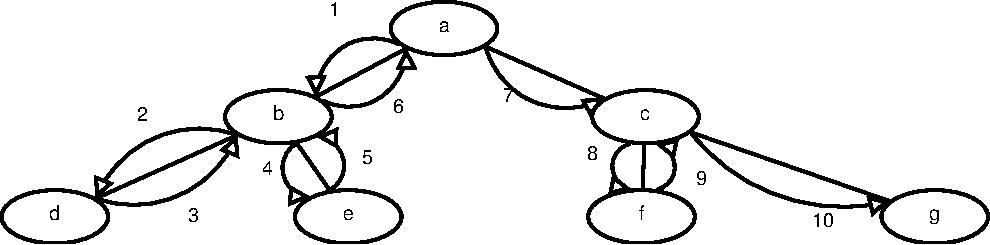
\includegraphics[width=0.7\linewidth]{images/preordem}
		\caption{Pré-ordem}
		\label{fig:preordem}
	\end{figure}
\end{frame}


\begin{frame}
	\frametitle{Algoritmos de busca em grafos}
	\framesubtitle{AVL - Árvore de busca balanceada - Algoritmos de percurso}
	\lstinputlisting[language=C++]{../codigo/percurso.cpp}
	
\end{frame}


\begin{frame}
	\frametitle{Algoritmos de busca em grafos}
	\framesubtitle{AVL - Árvore de busca balanceada - Algoritmo de balanceamento}
	\par Uma árvore binária, como já foi dito, pode degenerar em uma lista ligada sequencial prejudicando em muito o tempo de acesso aos seus dados. Para resolver isso se usa algumas técnicas de \textbf{rebalanceamento} da árvore.
\end{frame}

\begin{frame}
	\frametitle{Algoritmos de busca em grafos}
	\framesubtitle{AVL - Árvore de busca balanceada - Algoritmo de balanceamento}
	\begin{figure}
		\centering
		\includegraphics[width=0.7\linewidth]{images/AVLRotacaoAntiHoraria}
		\caption{Rotação anti-horária}
		\label{fig:avlrotacaoantihoraria}
	\end{figure}
	\begin{figure}
		\centering
		\includegraphics[width=0.7\linewidth]{images/AVLRotacaoHoraria}
		\caption{Rotação horária}
		\label{fig:avlrotacaohoraria}
	\end{figure}
\end{frame}

\begin{frame}
	\frametitle{Algoritmos de busca em grafos}
	\framesubtitle{AVL - Árvore de busca balanceada - Algoritmo de balanceamento}
	\par Baixe o código de \href{https://github.com/ensismoebius/1955SCC-Projeto-e-Analise-de-Algoritmos.git}{https://github.com/ensismoebius/1955SCC-Projeto-e-Analise-de-Algoritmos.git} e abra o projeto "arvoresEListas" lá você encontrará o arquivo \textit{main.cpp}. \textbf{Pergunta}: Qual o tempo de execução para adição e remoção de um item na AVL?
\end{frame}

\begin{frame}
	\frametitle{Algoritmos de busca em grafos}
	\framesubtitle{Árvores Trie}
	\par Uma Árvore Trie (termo definido em 1960 pelo professor Edward Fredkin a
	partir da abstração da palavra “retrieval”) pode ser descrita como uma estrutura de dados utilizada para armazenar de forma hierárquica cadeias de caracteres e suportar uma rápida procura de registros, sendo sua principal aplicação a procura por padrões	e prefixos. \newline
	\par O grande diferencial das Árvores Trie em relação as, por exemplo, árvores de busca binárias (ABB), é que o valor a ser armazenado (daqui em diante chamaremos esse valor de chave) não precisa ser totalmente guardado em alguma estrutura interna da árvore (nó), pois a própria estrutura da árvore Trie consegue representar senão	toda, boa parte da chave.
\end{frame}

\begin{frame}
	\frametitle{Algoritmos de busca em grafos}
	\framesubtitle{Árvores Trie}
	\par Organização dos dados em uma trie:
	\begin{itemize}
		\item dados não são guardados em apenas um nó
		\item dados são tratados como elementos divisíveis dispersos na árvore
		\item cada nó possui como valor implícito um caractere de um alfabeto pré-definido
		\item \textbf{prefixo de chave} é o caminho desde a raiz até um nó não-folha
	\end{itemize}
	\par O primeiro nível da trie é composto tão e somente por um único vetor, no qual é	colocado o primeiro caractere da chave que se pretende armazenar, caso a chave tenha mais de um caractere então será criado dinamicamente um outro vetor em um nível abaixo do primeiro, e, assim por diante até que todos os caracteres da chave	sejam mapeados.
\end{frame}

\begin{frame}
	\frametitle{Algoritmos de busca em grafos}
	\framesubtitle{Árvores Trie}
	\begin{columns}
		\begin{column}{0.7\textwidth}
			\begin{figure}
				\centering
				\includegraphics[width=\linewidth]{images/trie}
				\caption{Uma trie}
				\label{fig:trie}
			\end{figure}
		\end{column}
		\begin{column}{0.3\textwidth}
			\par Nós marcados em verde são as folhas da trie.
			\par Perceba que essa estrutura tem níveis.
			\par O que esses níveis tem de especial?
		\end{column}
	\end{columns}
\end{frame}

\begin{frame}
	\frametitle{Algoritmos de busca em grafos}
	\framesubtitle{Árvores Trie}
		\par Cada nó é representado usando uma estrutura como a abaixo:
		\begin{columns}
			\begin{column}{0.5\textwidth}
				\lstinputlisting[language=C++]{../codigo/trienode.h}
			\end{column}
			\begin{column}{0.5\textwidth}
				\lstinputlisting[language=C++]{../codigo/trienode.cpp}
			\end{column}
		\end{columns}
\end{frame}

\begin{frame}
	\frametitle{Algoritmos de busca em grafos}
	\framesubtitle{Árvores Trie}
	\par A trie com suas operações pode ser representada dessa forma:
	\lstinputlisting[language=C++]{../codigo/trie.h}
\end{frame}

\begin{frame}[allowframebreaks]
	\frametitle{Algoritmos de busca em grafos}
	\framesubtitle{Árvores Trie}
	\par A trie com suas operações pode ser representada dessa forma:
	\lstinputlisting[language=C++]{../codigo/trie.cpp}
\end{frame}


\begin{frame}
	\frametitle{Algoritmos de busca em grafos}
	\framesubtitle{Árvores Trie}
	\par \textbf{Exercício 1542660005445454545877:} Usando a trie crie um sistema que dado o \textbf{prefixo} de uma palavra o mesmo retorne todas as palavras cadastradas com aquele prefixo. Por exemplo: "par" $\rightarrow$ \textbf{par}angaricutirimiruaro, \textbf{par}aná, \textbf{par}cimônia, etc.
	\par Considerando que o tamanho da entrada $n$ é a quantidade de letras na palavra, qual o tempo de execução para \textbf{localizar uma palavra}?
	\par E quando a palavra não é encontrada?\newline
	\pause
	\par \textbf{Resposta}:
	\par $\Theta(n)$ e $O(n), \Omega(1)$
\end{frame}